\documentclass[twoside]{book}

% Packages required by doxygen
\usepackage{fixltx2e}
\usepackage{calc}
\usepackage{doxygen}
\usepackage{graphicx}
\usepackage[utf8]{inputenc}
\usepackage{makeidx}
\usepackage{multicol}
\usepackage{multirow}
\PassOptionsToPackage{warn}{textcomp}
\usepackage{textcomp}
\usepackage[nointegrals]{wasysym}
\usepackage[table]{xcolor}

% Font selection
\usepackage[T1]{fontenc}
\usepackage{mathptmx}
\usepackage[scaled=.90]{helvet}
\usepackage{courier}
\usepackage{amssymb}
\usepackage{sectsty}
\renewcommand{\familydefault}{\sfdefault}
\allsectionsfont{%
  \fontseries{bc}\selectfont%
  \color{darkgray}%
}
\renewcommand{\DoxyLabelFont}{%
  \fontseries{bc}\selectfont%
  \color{darkgray}%
}
\newcommand{\+}{\discretionary{\mbox{\scriptsize$\hookleftarrow$}}{}{}}

% Page & text layout
\usepackage{geometry}
\geometry{%
  a4paper,%
  top=2.5cm,%
  bottom=2.5cm,%
  left=2.5cm,%
  right=2.5cm%
}
\tolerance=750
\hfuzz=15pt
\hbadness=750
\setlength{\emergencystretch}{15pt}
\setlength{\parindent}{0cm}
\setlength{\parskip}{0.2cm}
\makeatletter
\renewcommand{\paragraph}{%
  \@startsection{paragraph}{4}{0ex}{-1.0ex}{1.0ex}{%
    \normalfont\normalsize\bfseries\SS@parafont%
  }%
}
\renewcommand{\subparagraph}{%
  \@startsection{subparagraph}{5}{0ex}{-1.0ex}{1.0ex}{%
    \normalfont\normalsize\bfseries\SS@subparafont%
  }%
}
\makeatother

% Headers & footers
\usepackage{fancyhdr}
\pagestyle{fancyplain}
\fancyhead[LE]{\fancyplain{}{\bfseries\thepage}}
\fancyhead[CE]{\fancyplain{}{}}
\fancyhead[RE]{\fancyplain{}{\bfseries\leftmark}}
\fancyhead[LO]{\fancyplain{}{\bfseries\rightmark}}
\fancyhead[CO]{\fancyplain{}{}}
\fancyhead[RO]{\fancyplain{}{\bfseries\thepage}}
\fancyfoot[LE]{\fancyplain{}{}}
\fancyfoot[CE]{\fancyplain{}{}}
\fancyfoot[RE]{\fancyplain{}{\bfseries\scriptsize Generated on Mon Apr 18 2016 22\+:27\+:19 for Andrew and Nick's Project by Doxygen }}
\fancyfoot[LO]{\fancyplain{}{\bfseries\scriptsize Generated on Mon Apr 18 2016 22\+:27\+:19 for Andrew and Nick's Project by Doxygen }}
\fancyfoot[CO]{\fancyplain{}{}}
\fancyfoot[RO]{\fancyplain{}{}}
\renewcommand{\footrulewidth}{0.4pt}
\renewcommand{\chaptermark}[1]{%
  \markboth{#1}{}%
}
\renewcommand{\sectionmark}[1]{%
  \markright{\thesection\ #1}%
}

% Indices & bibliography
\usepackage{natbib}
\usepackage[titles]{tocloft}
\setcounter{tocdepth}{3}
\setcounter{secnumdepth}{5}
\makeindex

% Hyperlinks (required, but should be loaded last)
\usepackage{ifpdf}
\ifpdf
  \usepackage[pdftex,pagebackref=true]{hyperref}
\else
  \usepackage[ps2pdf,pagebackref=true]{hyperref}
\fi
\hypersetup{%
  colorlinks=true,%
  linkcolor=blue,%
  citecolor=blue,%
  unicode%
}

% Custom commands
\newcommand{\clearemptydoublepage}{%
  \newpage{\pagestyle{empty}\cleardoublepage}%
}


%===== C O N T E N T S =====

\begin{document}

% Titlepage & ToC
\hypersetup{pageanchor=false,
             bookmarks=true,
             bookmarksnumbered=true,
             pdfencoding=unicode
            }
\pagenumbering{roman}
\begin{titlepage}
\vspace*{7cm}
\begin{center}%
{\Large Andrew and Nick's Project }\\
\vspace*{1cm}
{\large Generated by Doxygen 1.8.8}\\
\vspace*{0.5cm}
{\small Mon Apr 18 2016 22:27:19}\\
\end{center}
\end{titlepage}
\clearemptydoublepage
\tableofcontents
\clearemptydoublepage
\pagenumbering{arabic}
\hypersetup{pageanchor=true}

%--- Begin generated contents ---
\chapter{Namespace Index}
\section{Namespace List}
Here is a list of all namespaces with brief descriptions\+:\begin{DoxyCompactList}
\item\contentsline{section}{\hyperlink{namespacevaso}{vaso} \\*Function()s related to the program's threaded processing of audio data }{\pageref{namespacevaso}}{}
\end{DoxyCompactList}

\chapter{Class Index}
\section{Class List}
Here are the classes, structs, unions and interfaces with brief descriptions\+:\begin{DoxyCompactList}
\item\contentsline{section}{\hyperlink{structDataParams}{Data\+Params} }{\pageref{structDataParams}}{}
\item\contentsline{section}{\hyperlink{structMaximum}{Maximum} }{\pageref{structMaximum}}{}
\end{DoxyCompactList}

\chapter{File Index}
\section{File List}
Here is a list of all files with brief descriptions\+:\begin{DoxyCompactList}
\item\contentsline{section}{\hyperlink{makefile}{makefile} \\*Contains recipes for building the test applications, the main application, and the documentation }{\pageref{makefile}}{}
\item\contentsline{section}{etc/\hyperlink{doxygen_8config}{doxygen.\+config} \\*Contains Doxygen configuration settings }{\pageref{doxygen_8config}}{}
\item\contentsline{section}{src/\hyperlink{definitions_8hpp}{definitions.\+hpp} \\*Contains declarations of system-\/independant (universal size) integers and float types, shortened type names for some commonly used types, and enumerations }{\pageref{definitions_8hpp}}{}
\item\contentsline{section}{src/\hyperlink{fileio_8hpp}{fileio.\+hpp} \\*Functions related to the file I/\+O use in this program }{\pageref{fileio_8hpp}}{}
\item\contentsline{section}{src/\hyperlink{fileio__test_8cpp}{fileio\+\_\+test.\+cpp} \\*Contains program that tests the functions in \hyperlink{fileio_8hpp}{fileio.\+hpp} }{\pageref{fileio__test_8cpp}}{}
\item\contentsline{section}{src/\hyperlink{main_8cpp}{main.\+cpp} \\*Contains the main program }{\pageref{main_8cpp}}{}
\item\contentsline{section}{src/\hyperlink{patient__name__test_8cpp}{patient\+\_\+name\+\_\+test.\+cpp} \\*Contains a program to test the \hyperlink{namespaceavda_ae20728e7e8ae50bf2f74849e538841ea}{Patient\+Name()} function }{\pageref{patient__name__test_8cpp}}{}
\item\contentsline{section}{src/\hyperlink{process_8hpp}{process.\+hpp} \\*Contains functions related to the program's threaded processing of audio data }{\pageref{process_8hpp}}{}
\item\contentsline{section}{src/\hyperlink{process__test_8cpp}{process\+\_\+test.\+cpp} \\*Contains a program to test the \hyperlink{namespaceavda_a5196cce27286d08ca144a460caee7839}{process()} function }{\pageref{process__test_8cpp}}{}
\item\contentsline{section}{src/\hyperlink{read__params__test_8cpp}{read\+\_\+params\+\_\+test.\+cpp} \\*Contains a program test the \hyperlink{namespaceavda_ae20728e7e8ae50bf2f74849e538841ea}{Patient\+Name()} function }{\pageref{read__params__test_8cpp}}{}
\item\contentsline{section}{src/\hyperlink{sigmath_8hpp}{sigmath.\+hpp} \\*Functions necessary to perform the mathematical operations required by this program }{\pageref{sigmath_8hpp}}{}
\item\contentsline{section}{src/\hyperlink{sound_8hpp}{sound.\+hpp} \\*Function(s) relating to sound }{\pageref{sound_8hpp}}{}
\item\contentsline{section}{src/\hyperlink{stdin__clear__test_8cpp}{stdin\+\_\+clear\+\_\+test.\+cpp} \\*Contains a program to test clearing the stdin buffer }{\pageref{stdin__clear__test_8cpp}}{}
\end{DoxyCompactList}

\chapter{Namespace Documentation}
\hypertarget{namespacevaso}{\section{vaso Namespace Reference}
\label{namespacevaso}\index{vaso@{vaso}}
}


contains functions related to the file I/\+O use in this program  


\subsection*{Enumerations}
\begin{DoxyCompactItemize}
\item 
enum \hyperlink{namespacevaso_a77c5d9704657d49d456f691ddd8abf7c}{Side} \{ \hyperlink{namespacevaso_a77c5d9704657d49d456f691ddd8abf7ca945d5e233cf7d6240f6b783b36a374ff}{Side\+::\+Left}, 
\hyperlink{namespacevaso_a77c5d9704657d49d456f691ddd8abf7ca92b09c7c48c520c3c55e497875da437c}{Side\+::\+Right}
 \}
\end{DoxyCompactItemize}
\subsection*{Functions}
\begin{DoxyCompactItemize}
\item 
std\+::string \hyperlink{namespacevaso_abab641a332f2e834dfcdf294c0429426}{Current\+Data\+Name} ()
\item 
std\+::string \hyperlink{namespacevaso_af8f45524d4770053c2b812ce33a7095f}{Initial\+Data\+Name} (auto dir)
\item 
std\+::string \hyperlink{namespacevaso_a21e264fa912f7ca3f50e7e412ba1582e}{Patient\+Name} ()
\item 
\hyperlink{structDataParams}{Data\+Params} \hyperlink{namespacevaso_a6f1a23c617aae2e2c4af5e8016b4d03e}{Read\+Params} (auto filename)
\item 
std\+::string \hyperlink{namespacevaso_ad8543c0caabf3836b4a93a78e0d487d1}{Write\+Params} (\hyperlink{structDataParams}{Data\+Params} params, auto filename)
\item 
void \hyperlink{namespacevaso_a9d0e5d69685ee494d286db6ece005156}{average} (\hyperlink{definitions_8hpp_aacdc525d6f7bddb3ae95d5c311bd06a1}{float32} $\ast$data, \hyperlink{definitions_8hpp_aacdc525d6f7bddb3ae95d5c311bd06a1}{float32} $\ast$avg, \hyperlink{definitions_8hpp_adde6aaee8457bee49c2a92621fe22b79}{uint8} count, \hyperlink{definitions_8hpp_a1134b580f8da4de94ca6b1de4d37975e}{uint32} size)
\item 
void \hyperlink{namespacevaso_a7d108bce812e906d8b1810815774c7ea}{diff} (\hyperlink{definitions_8hpp_aacdc525d6f7bddb3ae95d5c311bd06a1}{float32} $\ast$data, \hyperlink{definitions_8hpp_a1134b580f8da4de94ca6b1de4d37975e}{uint32} size)
\item 
void \hyperlink{namespacevaso_af74f08a8afd7967b6c2b3c2b0e5fb1e9}{fft} (\hyperlink{definitions_8hpp_a960be6b6614c08090c16574dba10a421}{cfloat32} $\ast$data, \hyperlink{definitions_8hpp_a1134b580f8da4de94ca6b1de4d37975e}{uint32} size)
\item 
void \hyperlink{namespacevaso_a5d355b5c326a852e2ce95c258450898c}{mag} (\hyperlink{definitions_8hpp_a960be6b6614c08090c16574dba10a421}{cfloat32} $\ast$orig, \hyperlink{definitions_8hpp_aacdc525d6f7bddb3ae95d5c311bd06a1}{float32} $\ast$newmags, \hyperlink{definitions_8hpp_a1134b580f8da4de94ca6b1de4d37975e}{uint32} size)
\item 
void \hyperlink{namespacevaso_a649803d9dd74002f7975dba6b48b56ce}{max} (\hyperlink{definitions_8hpp_aacdc525d6f7bddb3ae95d5c311bd06a1}{float32} $\ast$data, \hyperlink{definitions_8hpp_a1134b580f8da4de94ca6b1de4d37975e}{uint32} size)
\item 
void \hyperlink{namespacevaso_a5b7fc1a58199e2cac989f417a9faa1ce}{smooth} (\hyperlink{definitions_8hpp_aacdc525d6f7bddb3ae95d5c311bd06a1}{float32} $\ast$data, \hyperlink{definitions_8hpp_a1134b580f8da4de94ca6b1de4d37975e}{uint32} size, \hyperlink{definitions_8hpp_a05f6b0ae8f6a6e135b0e290c25fe0e4e}{uint16} order)
\item 
void \hyperlink{namespacevaso_a7da499b9b1b5a492bea8ab8681e57c22}{play} (auto filename)
\item 
void $\ast$ \hyperlink{namespacevaso_acd767ffd09e8d7323a0275e8f88a6de2}{process} (void $\ast$procdata)
\item 
void \hyperlink{namespacevaso_aec526a2735f71ef68cea3e00ae943edf}{Start\+Processing} (\hyperlink{structProcData}{Proc\+Data} procdata)
\item 
void $\ast$ \hyperlink{namespacevaso_ae553d67666b43a570bbb1753b2a624d2}{processing} (void $\ast$procdata)
\end{DoxyCompactItemize}
\subsection*{Variables}
\begin{DoxyCompactItemize}
\item 
const std\+::string \hyperlink{namespacevaso_a0f49c8240a13e7d853912ad78d5f53c9}{P\+A\+T\+I\+E\+N\+T\+\_\+\+P\+A\+T\+H} = \char`\"{}/home/pi/patients/\char`\"{}
\end{DoxyCompactItemize}


\subsection{Detailed Description}
contains functions related to the file I/\+O use in this program 

contains functions related to the program's threaded processing of audio data

contains the function(s) relating to sound

contains the functions necessary to perform the mathematical operations required by this program

This namespace contains all code related to this project.

\begin{DoxyAuthor}{Author}
Samuel Andrew Wisner, \href{mailto:awisner94@gmail.com}{\tt awisner94@gmail.\+com}

Samuel Andrew Wisner, \href{mailto:awisner94@gmail.com}{\tt awisner94@gmail.\+com} 

Nicholas K. Nolan

Samuel Andrew Wisner, \href{mailto:awisne94@gmail.com}{\tt awisne94@gmail.\+com} 
\end{DoxyAuthor}


\subsection{Enumeration Type Documentation}
\hypertarget{namespacevaso_a77c5d9704657d49d456f691ddd8abf7c}{\index{vaso@{vaso}!Side@{Side}}
\index{Side@{Side}!vaso@{vaso}}
\subsubsection[{Side}]{\setlength{\rightskip}{0pt plus 5cm}enum {\bf vaso\+::\+Side}\hspace{0.3cm}{\ttfamily [strong]}}}\label{namespacevaso_a77c5d9704657d49d456f691ddd8abf7c}
The side of the head to which a recording pertains. \begin{Desc}
\item[Enumerator]\par
\begin{description}
\index{Left@{Left}!vaso@{vaso}}\index{vaso@{vaso}!Left@{Left}}\item[{\em 
\hypertarget{namespacevaso_a77c5d9704657d49d456f691ddd8abf7ca945d5e233cf7d6240f6b783b36a374ff}{Left}\label{namespacevaso_a77c5d9704657d49d456f691ddd8abf7ca945d5e233cf7d6240f6b783b36a374ff}
}]\index{Right@{Right}!vaso@{vaso}}\index{vaso@{vaso}!Right@{Right}}\item[{\em 
\hypertarget{namespacevaso_a77c5d9704657d49d456f691ddd8abf7ca92b09c7c48c520c3c55e497875da437c}{Right}\label{namespacevaso_a77c5d9704657d49d456f691ddd8abf7ca92b09c7c48c520c3c55e497875da437c}
}]\end{description}
\end{Desc}


Definition at line 58 of file definitions.\+hpp.



\subsection{Function Documentation}
\hypertarget{namespacevaso_a9d0e5d69685ee494d286db6ece005156}{\index{vaso@{vaso}!average@{average}}
\index{average@{average}!vaso@{vaso}}
\subsubsection[{average}]{\setlength{\rightskip}{0pt plus 5cm}void vaso\+::average (
\begin{DoxyParamCaption}
\item[{{\bf float32} $\ast$}]{data, }
\item[{{\bf float32} $\ast$}]{avg, }
\item[{{\bf uint8}}]{count, }
\item[{{\bf uint32}}]{size}
\end{DoxyParamCaption}
)}}\label{namespacevaso_a9d0e5d69685ee494d286db6ece005156}
Element-\/wise averaging along the first dimension of a two-\/dimensional array.


\begin{DoxyParams}{Parameters}
{\em data} & the two-\/dimensional array containing \mbox{[}count\mbox{]} number of arrays in the first dimension and \mbox{[}size\mbox{]} number of each elements in the second dimension\\
\hline
{\em avg} & the array of size \mbox{[}size\mbox{]} containing the averaged values of each element\\
\hline
{\em count} & the number of arrays in the first dimension of data and will likely be a constant value of 3 in this program\\
\hline
{\em size} & the number of elements in the second dimension of data \\
\hline
\end{DoxyParams}


Definition at line 94 of file sigmath.\+hpp.

\hypertarget{namespacevaso_abab641a332f2e834dfcdf294c0429426}{\index{vaso@{vaso}!Current\+Data\+Name@{Current\+Data\+Name}}
\index{Current\+Data\+Name@{Current\+Data\+Name}!vaso@{vaso}}
\subsubsection[{Current\+Data\+Name}]{\setlength{\rightskip}{0pt plus 5cm}std\+::string vaso\+::\+Current\+Data\+Name (
\begin{DoxyParamCaption}
{}
\end{DoxyParamCaption}
)}}\label{namespacevaso_abab641a332f2e834dfcdf294c0429426}
Gets a data-\/based name to which the file(s) created in a session to be saved.

\begin{DoxyReturn}{Returns}
a partial (?) filename for the current session 
\end{DoxyReturn}


Definition at line 26 of file fileio.\+hpp.

\hypertarget{namespacevaso_a7d108bce812e906d8b1810815774c7ea}{\index{vaso@{vaso}!diff@{diff}}
\index{diff@{diff}!vaso@{vaso}}
\subsubsection[{diff}]{\setlength{\rightskip}{0pt plus 5cm}void vaso\+::diff (
\begin{DoxyParamCaption}
\item[{{\bf float32} $\ast$}]{data, }
\item[{{\bf uint32}}]{size}
\end{DoxyParamCaption}
)}}\label{namespacevaso_a7d108bce812e906d8b1810815774c7ea}
Computes the left-\/handed first derivative of a discrete signal. The first element will be 0.


\begin{DoxyParams}{Parameters}
{\em data} & an array containing the discrete signal data\\
\hline
{\em size} & the number of elements in data \\
\hline
\end{DoxyParams}


Definition at line 98 of file sigmath.\+hpp.

\hypertarget{namespacevaso_af74f08a8afd7967b6c2b3c2b0e5fb1e9}{\index{vaso@{vaso}!fft@{fft}}
\index{fft@{fft}!vaso@{vaso}}
\subsubsection[{fft}]{\setlength{\rightskip}{0pt plus 5cm}void vaso\+::fft (
\begin{DoxyParamCaption}
\item[{{\bf cfloat32} $\ast$}]{data, }
\item[{{\bf uint32}}]{size}
\end{DoxyParamCaption}
)}}\label{namespacevaso_af74f08a8afd7967b6c2b3c2b0e5fb1e9}
Replaces the values of an array of cfloat32's with the array's D\+F\+T using a decimation-\/in-\/frequency algorithm.

This code is based on code from \href{http://rosettacode.org/wiki/Fast_Fourier_transform#C.2B.2B}{\tt http\+://rosettacode.\+org/wiki/\+Fast\+\_\+\+Fourier\+\_\+transform\#\+C.\+2\+B.\+2\+B}.


\begin{DoxyParams}{Parameters}
{\em data} & the array whose values should be replaced with its D\+F\+T\\
\hline
{\em size} & the number of elements in the data array \\
\hline
\end{DoxyParams}


Definition at line 102 of file sigmath.\+hpp.

\hypertarget{namespacevaso_af8f45524d4770053c2b812ce33a7095f}{\index{vaso@{vaso}!Initial\+Data\+Name@{Initial\+Data\+Name}}
\index{Initial\+Data\+Name@{Initial\+Data\+Name}!vaso@{vaso}}
\subsubsection[{Initial\+Data\+Name}]{\setlength{\rightskip}{0pt plus 5cm}std\+::string vaso\+::\+Initial\+Data\+Name (
\begin{DoxyParamCaption}
\item[{auto}]{dir}
\end{DoxyParamCaption}
)}}\label{namespacevaso_af8f45524d4770053c2b812ce33a7095f}
Finds the filename of the oldest (i.\+e., baseline) data is saved.


\begin{DoxyParams}{Parameters}
{\em dir} & the directory which contains all patient data\\
\hline
\end{DoxyParams}
\begin{DoxyReturn}{Returns}
the base (?) filename to which all baseline data was saved 
\end{DoxyReturn}


Definition at line 37 of file fileio.\+hpp.

\hypertarget{namespacevaso_a5d355b5c326a852e2ce95c258450898c}{\index{vaso@{vaso}!mag@{mag}}
\index{mag@{mag}!vaso@{vaso}}
\subsubsection[{mag}]{\setlength{\rightskip}{0pt plus 5cm}void vaso\+::mag (
\begin{DoxyParamCaption}
\item[{{\bf cfloat32} $\ast$}]{orig, }
\item[{{\bf float32} $\ast$}]{newmags, }
\item[{{\bf uint32}}]{size}
\end{DoxyParamCaption}
)}}\label{namespacevaso_a5d355b5c326a852e2ce95c258450898c}
Computes the magitude of an array of complex numbers.


\begin{DoxyParams}{Parameters}
{\em orig} & the array of complex numbers\\
\hline
{\em newmags} & an array to which the magitudes are to be written\\
\hline
{\em size} & the number of elements in orig and newmags \\
\hline
\end{DoxyParams}


Definition at line 150 of file sigmath.\+hpp.

\hypertarget{namespacevaso_a649803d9dd74002f7975dba6b48b56ce}{\index{vaso@{vaso}!max@{max}}
\index{max@{max}!vaso@{vaso}}
\subsubsection[{max}]{\setlength{\rightskip}{0pt plus 5cm}void vaso\+::max (
\begin{DoxyParamCaption}
\item[{{\bf float32} $\ast$}]{data, }
\item[{{\bf uint32}}]{size}
\end{DoxyParamCaption}
)}}\label{namespacevaso_a649803d9dd74002f7975dba6b48b56ce}
Finds the maximum value in an array.


\begin{DoxyParams}{Parameters}
{\em data} & the array whose maximum value is to be found\\
\hline
{\em uint32} & size the number of elements in the data array \\
\hline
\end{DoxyParams}


Definition at line 154 of file sigmath.\+hpp.

\hypertarget{namespacevaso_a21e264fa912f7ca3f50e7e412ba1582e}{\index{vaso@{vaso}!Patient\+Name@{Patient\+Name}}
\index{Patient\+Name@{Patient\+Name}!vaso@{vaso}}
\subsubsection[{Patient\+Name}]{\setlength{\rightskip}{0pt plus 5cm}std\+::string vaso\+::\+Patient\+Name (
\begin{DoxyParamCaption}
{}
\end{DoxyParamCaption}
)}}\label{namespacevaso_a21e264fa912f7ca3f50e7e412ba1582e}
Prompts a user to enter a first, middle, and last name for a patients and creates a directory (if necessary) in which all of a patient's data can be saved.

Must warn a user if the patient folder does not already exist in order to prevent missaving data.

\begin{DoxyReturn}{Returns}
the directory under which all patient data is saved 
\end{DoxyReturn}


Definition at line 51 of file fileio.\+hpp.

\hypertarget{namespacevaso_a7da499b9b1b5a492bea8ab8681e57c22}{\index{vaso@{vaso}!play@{play}}
\index{play@{play}!vaso@{vaso}}
\subsubsection[{play}]{\setlength{\rightskip}{0pt plus 5cm}void vaso\+::play (
\begin{DoxyParamCaption}
\item[{auto}]{filename}
\end{DoxyParamCaption}
)}}\label{namespacevaso_a7da499b9b1b5a492bea8ab8681e57c22}
Plays a W\+A\+V\+E file in a loop in a non-\/blocking manner.


\begin{DoxyParams}{Parameters}
{\em filename} & the absolute or relative path to the W\+A\+V\+E file \\
\hline
\end{DoxyParams}


Definition at line 19 of file sound.\+hpp.

\hypertarget{namespacevaso_acd767ffd09e8d7323a0275e8f88a6de2}{\index{vaso@{vaso}!process@{process}}
\index{process@{process}!vaso@{vaso}}
\subsubsection[{process}]{\setlength{\rightskip}{0pt plus 5cm}void$\ast$ vaso\+::process (
\begin{DoxyParamCaption}
\item[{void $\ast$}]{procdata}
\end{DoxyParamCaption}
)}}\label{namespacevaso_acd767ffd09e8d7323a0275e8f88a6de2}
Computes recording parameters in a separate thread in a thread-\/safe manner. A\+Utomatically waits for each recording to finish before processing it. This file is meant to be called O\+N\+L\+Y from the Start\+Processing function.


\begin{DoxyParams}{Parameters}
{\em procdata} & a struct containing the values necessary to processing the audio\\
\hline
\end{DoxyParams}
\begin{DoxyReturn}{Returns}
a (void) pointer to a \hyperlink{structDataParams}{Data\+Params} struct containing the computed parameters for a patient 
\end{DoxyReturn}
\hypertarget{namespacevaso_ae553d67666b43a570bbb1753b2a624d2}{\index{vaso@{vaso}!processing@{processing}}
\index{processing@{processing}!vaso@{vaso}}
\subsubsection[{processing}]{\setlength{\rightskip}{0pt plus 5cm}void$\ast$ vaso\+::processing (
\begin{DoxyParamCaption}
\item[{void $\ast$}]{procdata}
\end{DoxyParamCaption}
)}}\label{namespacevaso_ae553d67666b43a570bbb1753b2a624d2}


Definition at line 42 of file threadproc.\+hpp.

\hypertarget{namespacevaso_a6f1a23c617aae2e2c4af5e8016b4d03e}{\index{vaso@{vaso}!Read\+Params@{Read\+Params}}
\index{Read\+Params@{Read\+Params}!vaso@{vaso}}
\subsubsection[{Read\+Params}]{\setlength{\rightskip}{0pt plus 5cm}{\bf Data\+Params} vaso\+::\+Read\+Params (
\begin{DoxyParamCaption}
\item[{auto}]{filename}
\end{DoxyParamCaption}
)}}\label{namespacevaso_a6f1a23c617aae2e2c4af5e8016b4d03e}
Reads the previously computated parameters found in the specified file.


\begin{DoxyParams}{Parameters}
{\em filename} & the absolute or relative path to the file containing the patient data to read\\
\hline
\end{DoxyParams}
\begin{DoxyReturn}{Returns}
the patient parameters read 
\end{DoxyReturn}


Definition at line 64 of file fileio.\+hpp.

\hypertarget{namespacevaso_a5b7fc1a58199e2cac989f417a9faa1ce}{\index{vaso@{vaso}!smooth@{smooth}}
\index{smooth@{smooth}!vaso@{vaso}}
\subsubsection[{smooth}]{\setlength{\rightskip}{0pt plus 5cm}void vaso\+::smooth (
\begin{DoxyParamCaption}
\item[{{\bf float32} $\ast$}]{data, }
\item[{{\bf uint32}}]{size, }
\item[{{\bf uint16}}]{order}
\end{DoxyParamCaption}
)}}\label{namespacevaso_a5b7fc1a58199e2cac989f417a9faa1ce}
Applies an nth-\/order moving-\/average filter to a discrete signal.


\begin{DoxyParams}{Parameters}
{\em data} & the array containing the signal to which the filter should be applied\\
\hline
{\em size} & the number of elements in the data array\\
\hline
{\em order} & the order of the filter \\
\hline
\end{DoxyParams}


Definition at line 158 of file sigmath.\+hpp.

\hypertarget{namespacevaso_aec526a2735f71ef68cea3e00ae943edf}{\index{vaso@{vaso}!Start\+Processing@{Start\+Processing}}
\index{Start\+Processing@{Start\+Processing}!vaso@{vaso}}
\subsubsection[{Start\+Processing}]{\setlength{\rightskip}{0pt plus 5cm}void vaso\+::\+Start\+Processing (
\begin{DoxyParamCaption}
\item[{{\bf Proc\+Data}}]{procdata}
\end{DoxyParamCaption}
)}}\label{namespacevaso_aec526a2735f71ef68cea3e00ae943edf}
Begins processing the recorded data. Should be called before or immediately after the first recording.


\begin{DoxyParams}{Parameters}
{\em proxdata} & a struct containing the values necessary to processing the audio \\
\hline
\end{DoxyParams}


Definition at line 46 of file threadproc.\+hpp.

\hypertarget{namespacevaso_ad8543c0caabf3836b4a93a78e0d487d1}{\index{vaso@{vaso}!Write\+Params@{Write\+Params}}
\index{Write\+Params@{Write\+Params}!vaso@{vaso}}
\subsubsection[{Write\+Params}]{\setlength{\rightskip}{0pt plus 5cm}std\+::string vaso\+::\+Write\+Params (
\begin{DoxyParamCaption}
\item[{{\bf Data\+Params}}]{params, }
\item[{auto}]{filename}
\end{DoxyParamCaption}
)}}\label{namespacevaso_ad8543c0caabf3836b4a93a78e0d487d1}
Writes the parameters to the specified file.


\begin{DoxyParams}{Parameters}
{\em params} & \\
\hline
\end{DoxyParams}


Definition at line 73 of file fileio.\+hpp.



\subsection{Variable Documentation}
\hypertarget{namespacevaso_a0f49c8240a13e7d853912ad78d5f53c9}{\index{vaso@{vaso}!P\+A\+T\+I\+E\+N\+T\+\_\+\+P\+A\+T\+H@{P\+A\+T\+I\+E\+N\+T\+\_\+\+P\+A\+T\+H}}
\index{P\+A\+T\+I\+E\+N\+T\+\_\+\+P\+A\+T\+H@{P\+A\+T\+I\+E\+N\+T\+\_\+\+P\+A\+T\+H}!vaso@{vaso}}
\subsubsection[{P\+A\+T\+I\+E\+N\+T\+\_\+\+P\+A\+T\+H}]{\setlength{\rightskip}{0pt plus 5cm}const std\+::string vaso\+::\+P\+A\+T\+I\+E\+N\+T\+\_\+\+P\+A\+T\+H = \char`\"{}/home/pi/patients/\char`\"{}}}\label{namespacevaso_a0f49c8240a13e7d853912ad78d5f53c9}
Absolute path to the folder containing the patients' data 

Definition at line 18 of file fileio.\+hpp.


\chapter{Class Documentation}
\hypertarget{structDataParams}{\section{Data\+Params Struct Reference}
\label{structDataParams}\index{Data\+Params@{Data\+Params}}
}


{\ttfamily \#include $<$definitions.\+hpp$>$}



\subsection{Detailed Description}
A structure containing the calculated results from processing the audio recordings. 

Definition at line 40 of file definitions.\+hpp.



The documentation for this struct was generated from the following file\+:\begin{DoxyCompactItemize}
\item 
src/\hyperlink{definitions_8hpp}{definitions.\+hpp}\end{DoxyCompactItemize}

\hypertarget{structMaximum}{\section{Maximum Struct Reference}
\label{structMaximum}\index{Maximum@{Maximum}}
}


{\ttfamily \#include $<$definitions.\+hpp$>$}

\subsection*{Public Attributes}
\begin{DoxyCompactItemize}
\item 
\hyperlink{definitions_8hpp_aacdc525d6f7bddb3ae95d5c311bd06a1}{float32} \hyperlink{structMaximum_aa7e84cbf37b694670142670014366969}{value}
\item 
\hyperlink{definitions_8hpp_a1134b580f8da4de94ca6b1de4d37975e}{uint32} \hyperlink{structMaximum_a2e6aef03795cd285fe542d0861c6e3b5}{index}
\end{DoxyCompactItemize}


\subsection{Detailed Description}
Contains the maximum value found in an array and the value's index in that array. 

Definition at line \hyperlink{definitions_8hpp_source_l00053}{53} of file \hyperlink{definitions_8hpp_source}{definitions.\+hpp}.



\subsection{Member Data Documentation}
\hypertarget{structMaximum_a2e6aef03795cd285fe542d0861c6e3b5}{\index{Maximum@{Maximum}!index@{index}}
\index{index@{index}!Maximum@{Maximum}}
\subsubsection[{index}]{\setlength{\rightskip}{0pt plus 5cm}{\bf uint32} Maximum\+::index}}\label{structMaximum_a2e6aef03795cd285fe542d0861c6e3b5}


Definition at line \hyperlink{definitions_8hpp_source_l00055}{55} of file \hyperlink{definitions_8hpp_source}{definitions.\+hpp}.

\hypertarget{structMaximum_aa7e84cbf37b694670142670014366969}{\index{Maximum@{Maximum}!value@{value}}
\index{value@{value}!Maximum@{Maximum}}
\subsubsection[{value}]{\setlength{\rightskip}{0pt plus 5cm}{\bf float32} Maximum\+::value}}\label{structMaximum_aa7e84cbf37b694670142670014366969}


Definition at line \hyperlink{definitions_8hpp_source_l00054}{54} of file \hyperlink{definitions_8hpp_source}{definitions.\+hpp}.



The documentation for this struct was generated from the following file\+:\begin{DoxyCompactItemize}
\item 
src/\hyperlink{definitions_8hpp}{definitions.\+hpp}\end{DoxyCompactItemize}

\hypertarget{structThreadParams}{\section{Thread\+Params Struct Reference}
\label{structThreadParams}\index{Thread\+Params@{Thread\+Params}}
}


{\ttfamily \#include $<$definitions.\+hpp$>$}

\subsection*{Public Attributes}
\begin{DoxyCompactItemize}
\item 
\hyperlink{definitions_8hpp_aacdc525d6f7bddb3ae95d5c311bd06a1}{float32} $\ast$$\ast$ \hyperlink{structThreadParams_a94da463ea449a9fe597b442be56844b9}{data}
\item 
\hyperlink{definitions_8hpp_adde6aaee8457bee49c2a92621fe22b79}{uint8} \hyperlink{structThreadParams_a02e6a905a01a79e8b73fbe21318f82b0}{rec\+Count}
\item 
\hyperlink{definitions_8hpp_a1134b580f8da4de94ca6b1de4d37975e}{uint32} \hyperlink{structThreadParams_ad953eac404cb1fe5057bb6e8fd8bf63f}{sample\+Count}
\item 
\hyperlink{definitions_8hpp_a1134b580f8da4de94ca6b1de4d37975e}{uint32} \hyperlink{structThreadParams_a4c35a854b35945bda8ce13c01123e420}{sample\+Freq}
\item 
\hyperlink{definitions_8hpp_adde6aaee8457bee49c2a92621fe22b79}{uint8} $\ast$ \hyperlink{structThreadParams_aa23fd1fa0f6a8d38cb42d8ee852bc6a6}{counter}
\item 
std\+::map$<$ \hyperlink{namespacevaso_a77c5d9704657d49d456f691ddd8abf7c}{vaso\+::\+Side}, \hyperlink{structDataParams}{Data\+Params} $>$ \hyperlink{structThreadParams_a2332b920eca7ca1fa61cc078e99e0668}{results}
\end{DoxyCompactItemize}


\subsection{Detailed Description}
Contains the information needed by the thread that executes the \hyperlink{namespacevaso_a852067e19b0bcfebb4fa6674c7c8d67f}{Process()} function. 

Definition at line \hyperlink{definitions_8hpp_source_l00072}{72} of file \hyperlink{definitions_8hpp_source}{definitions.\+hpp}.



\subsection{Member Data Documentation}
\hypertarget{structThreadParams_aa23fd1fa0f6a8d38cb42d8ee852bc6a6}{\index{Thread\+Params@{Thread\+Params}!counter@{counter}}
\index{counter@{counter}!Thread\+Params@{Thread\+Params}}
\subsubsection[{counter}]{\setlength{\rightskip}{0pt plus 5cm}{\bf uint8}$\ast$ Thread\+Params\+::counter}}\label{structThreadParams_aa23fd1fa0f6a8d38cb42d8ee852bc6a6}


Definition at line \hyperlink{definitions_8hpp_source_l00077}{77} of file \hyperlink{definitions_8hpp_source}{definitions.\+hpp}.

\hypertarget{structThreadParams_a94da463ea449a9fe597b442be56844b9}{\index{Thread\+Params@{Thread\+Params}!data@{data}}
\index{data@{data}!Thread\+Params@{Thread\+Params}}
\subsubsection[{data}]{\setlength{\rightskip}{0pt plus 5cm}{\bf float32}$\ast$$\ast$ Thread\+Params\+::data}}\label{structThreadParams_a94da463ea449a9fe597b442be56844b9}


Definition at line \hyperlink{definitions_8hpp_source_l00073}{73} of file \hyperlink{definitions_8hpp_source}{definitions.\+hpp}.

\hypertarget{structThreadParams_a02e6a905a01a79e8b73fbe21318f82b0}{\index{Thread\+Params@{Thread\+Params}!rec\+Count@{rec\+Count}}
\index{rec\+Count@{rec\+Count}!Thread\+Params@{Thread\+Params}}
\subsubsection[{rec\+Count}]{\setlength{\rightskip}{0pt plus 5cm}{\bf uint8} Thread\+Params\+::rec\+Count}}\label{structThreadParams_a02e6a905a01a79e8b73fbe21318f82b0}


Definition at line \hyperlink{definitions_8hpp_source_l00074}{74} of file \hyperlink{definitions_8hpp_source}{definitions.\+hpp}.

\hypertarget{structThreadParams_a2332b920eca7ca1fa61cc078e99e0668}{\index{Thread\+Params@{Thread\+Params}!results@{results}}
\index{results@{results}!Thread\+Params@{Thread\+Params}}
\subsubsection[{results}]{\setlength{\rightskip}{0pt plus 5cm}std\+::map$<${\bf vaso\+::\+Side}, {\bf Data\+Params}$>$ Thread\+Params\+::results}}\label{structThreadParams_a2332b920eca7ca1fa61cc078e99e0668}


Definition at line \hyperlink{definitions_8hpp_source_l00078}{78} of file \hyperlink{definitions_8hpp_source}{definitions.\+hpp}.

\hypertarget{structThreadParams_ad953eac404cb1fe5057bb6e8fd8bf63f}{\index{Thread\+Params@{Thread\+Params}!sample\+Count@{sample\+Count}}
\index{sample\+Count@{sample\+Count}!Thread\+Params@{Thread\+Params}}
\subsubsection[{sample\+Count}]{\setlength{\rightskip}{0pt plus 5cm}{\bf uint32} Thread\+Params\+::sample\+Count}}\label{structThreadParams_ad953eac404cb1fe5057bb6e8fd8bf63f}


Definition at line \hyperlink{definitions_8hpp_source_l00075}{75} of file \hyperlink{definitions_8hpp_source}{definitions.\+hpp}.

\hypertarget{structThreadParams_a4c35a854b35945bda8ce13c01123e420}{\index{Thread\+Params@{Thread\+Params}!sample\+Freq@{sample\+Freq}}
\index{sample\+Freq@{sample\+Freq}!Thread\+Params@{Thread\+Params}}
\subsubsection[{sample\+Freq}]{\setlength{\rightskip}{0pt plus 5cm}{\bf uint32} Thread\+Params\+::sample\+Freq}}\label{structThreadParams_a4c35a854b35945bda8ce13c01123e420}


Definition at line \hyperlink{definitions_8hpp_source_l00076}{76} of file \hyperlink{definitions_8hpp_source}{definitions.\+hpp}.



The documentation for this struct was generated from the following file\+:\begin{DoxyCompactItemize}
\item 
src/\hyperlink{definitions_8hpp}{definitions.\+hpp}\end{DoxyCompactItemize}

\chapter{File Documentation}
\hypertarget{definitions_8hpp}{\section{src/definitions.hpp File Reference}
\label{definitions_8hpp}\index{src/definitions.\+hpp@{src/definitions.\+hpp}}
}
{\ttfamily \#include $<$complex$>$}\\*
{\ttfamily \#include $<$map$>$}\\*
Include dependency graph for definitions.\+hpp\+:
\nopagebreak
\begin{figure}[H]
\begin{center}
\leavevmode
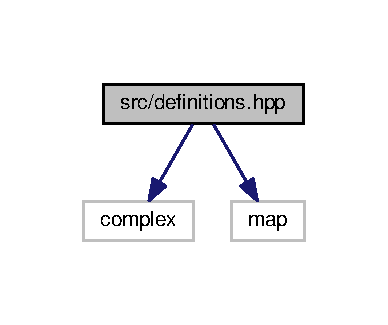
\includegraphics[width=186pt]{definitions_8hpp__incl}
\end{center}
\end{figure}
This graph shows which files directly or indirectly include this file\+:
\nopagebreak
\begin{figure}[H]
\begin{center}
\leavevmode
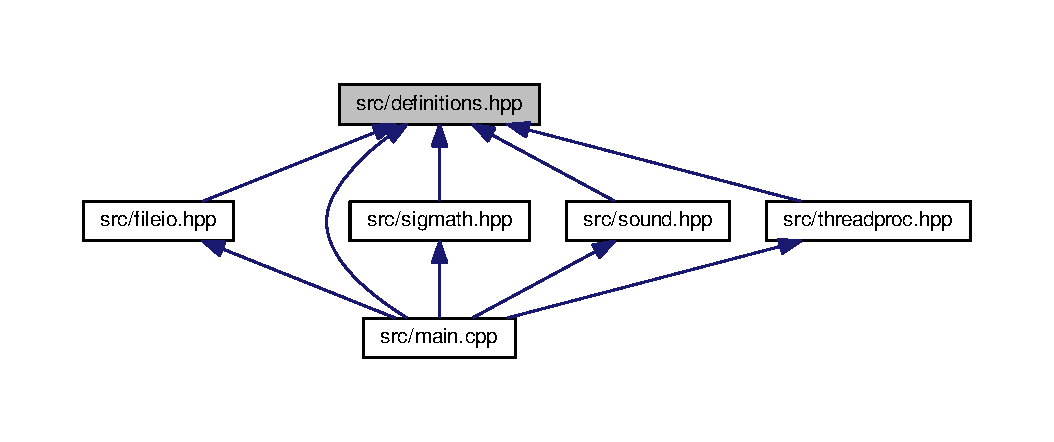
\includegraphics[width=350pt]{definitions_8hpp__dep__incl}
\end{center}
\end{figure}
\subsection*{Classes}
\begin{DoxyCompactItemize}
\item 
struct \hyperlink{structDataParams}{Data\+Params}
\item 
struct \hyperlink{structMaximum}{Maximum}
\item 
struct \hyperlink{structThreadParams}{Thread\+Params}
\end{DoxyCompactItemize}
\subsection*{Namespaces}
\begin{DoxyCompactItemize}
\item 
 \hyperlink{namespacevaso}{vaso}
\begin{DoxyCompactList}\small\item\em contains functions related to the file I/\+O use in this program \end{DoxyCompactList}\end{DoxyCompactItemize}
\subsection*{Macros}
\begin{DoxyCompactItemize}
\item 
\#define \hyperlink{definitions_8hpp_a8fe83ac76edc595f6b98cd4a4127aed5}{E\+R\+R\+O\+R}~-\/1
\begin{DoxyCompactList}\small\item\em Contains declarations of system-\/independant (universal size) integers and float types, shortened type names for some commonly used types, and enumerations. \end{DoxyCompactList}\item 
\#define \hyperlink{definitions_8hpp_aa44e6143be9e89f19be973956c22e134}{R\+E\+C\+\_\+\+C\+O\+U\+N\+T}~8
\item 
\#define \hyperlink{definitions_8hpp_a1682c770d91c5d167b621a782be940d4}{S\+A\+M\+P\+L\+E\+\_\+\+C\+O\+U\+N\+T}~262144
\item 
\#define \hyperlink{definitions_8hpp_a9401e43a8c86acafb31c8e2709baefa1}{S\+A\+M\+P\+L\+E\+\_\+\+F\+R\+E\+Q}~48000
\item 
\#define \hyperlink{definitions_8hpp_a378181c29a641d58f55d647b5a9599f2}{E\+N\+U\+M}~signed char
\end{DoxyCompactItemize}
\subsection*{Typedefs}
\begin{DoxyCompactItemize}
\item 
typedef unsigned char \hyperlink{definitions_8hpp_a0c8186d9b9b7880309c27230bbb5e69d}{byte}
\item 
typedef unsigned char \hyperlink{definitions_8hpp_adde6aaee8457bee49c2a92621fe22b79}{uint8}
\item 
typedef signed char \hyperlink{definitions_8hpp_a1a6408291ee3cfd0760a61ac64084154}{sint8}
\item 
typedef unsigned short \hyperlink{definitions_8hpp_a05f6b0ae8f6a6e135b0e290c25fe0e4e}{uint16}
\item 
typedef signed short \hyperlink{definitions_8hpp_a74df79fde3c518e55b29ce6360a9c76e}{sint16}
\item 
typedef unsigned int \hyperlink{definitions_8hpp_a1134b580f8da4de94ca6b1de4d37975e}{uint32}
\item 
typedef signed int \hyperlink{definitions_8hpp_a0573de65958b4fda3a0460ed417dafb8}{sint32}
\item 
typedef unsigned long long \hyperlink{definitions_8hpp_a29940ae63ec06c9998bba873e25407ad}{uint64}
\item 
typedef signed long long \hyperlink{definitions_8hpp_ad91d7e42d1c1abce1d9eeacd54cc0497}{sint64}
\item 
typedef float \hyperlink{definitions_8hpp_aacdc525d6f7bddb3ae95d5c311bd06a1}{float32}
\item 
typedef double \hyperlink{definitions_8hpp_a232fad1b0d6dcc7c16aabde98b2e2a80}{float64}
\item 
typedef std\+::complex$<$ \hyperlink{definitions_8hpp_aacdc525d6f7bddb3ae95d5c311bd06a1}{float32} $>$ \hyperlink{definitions_8hpp_a960be6b6614c08090c16574dba10a421}{cfloat32}
\end{DoxyCompactItemize}
\subsection*{Enumerations}
\begin{DoxyCompactItemize}
\item 
enum \hyperlink{namespacevaso_a77c5d9704657d49d456f691ddd8abf7c}{vaso\+::\+Side} \{ \hyperlink{namespacevaso_a77c5d9704657d49d456f691ddd8abf7ca945d5e233cf7d6240f6b783b36a374ff}{vaso\+::\+Side\+::\+Left}, 
\hyperlink{namespacevaso_a77c5d9704657d49d456f691ddd8abf7ca92b09c7c48c520c3c55e497875da437c}{vaso\+::\+Side\+::\+Right}
 \}
\end{DoxyCompactItemize}


\subsection{Macro Definition Documentation}
\hypertarget{definitions_8hpp_a378181c29a641d58f55d647b5a9599f2}{\index{definitions.\+hpp@{definitions.\+hpp}!E\+N\+U\+M@{E\+N\+U\+M}}
\index{E\+N\+U\+M@{E\+N\+U\+M}!definitions.\+hpp@{definitions.\+hpp}}
\subsubsection[{E\+N\+U\+M}]{\setlength{\rightskip}{0pt plus 5cm}\#define E\+N\+U\+M~signed char}}\label{definitions_8hpp_a378181c29a641d58f55d647b5a9599f2}


Definition at line \hyperlink{definitions_8hpp_source_l00018}{18} of file \hyperlink{definitions_8hpp_source}{definitions.\+hpp}.

\hypertarget{definitions_8hpp_a8fe83ac76edc595f6b98cd4a4127aed5}{\index{definitions.\+hpp@{definitions.\+hpp}!E\+R\+R\+O\+R@{E\+R\+R\+O\+R}}
\index{E\+R\+R\+O\+R@{E\+R\+R\+O\+R}!definitions.\+hpp@{definitions.\+hpp}}
\subsubsection[{E\+R\+R\+O\+R}]{\setlength{\rightskip}{0pt plus 5cm}\#define E\+R\+R\+O\+R~-\/1}}\label{definitions_8hpp_a8fe83ac76edc595f6b98cd4a4127aed5}


Contains declarations of system-\/independant (universal size) integers and float types, shortened type names for some commonly used types, and enumerations. 

\begin{DoxyAuthor}{Author}
Samuel Andrew Wisner, \href{mailto:awisner94@gmail.com}{\tt awisner94@gmail.\+com} 
\end{DoxyAuthor}


Definition at line \hyperlink{definitions_8hpp_source_l00014}{14} of file \hyperlink{definitions_8hpp_source}{definitions.\+hpp}.

\hypertarget{definitions_8hpp_aa44e6143be9e89f19be973956c22e134}{\index{definitions.\+hpp@{definitions.\+hpp}!R\+E\+C\+\_\+\+C\+O\+U\+N\+T@{R\+E\+C\+\_\+\+C\+O\+U\+N\+T}}
\index{R\+E\+C\+\_\+\+C\+O\+U\+N\+T@{R\+E\+C\+\_\+\+C\+O\+U\+N\+T}!definitions.\+hpp@{definitions.\+hpp}}
\subsubsection[{R\+E\+C\+\_\+\+C\+O\+U\+N\+T}]{\setlength{\rightskip}{0pt plus 5cm}\#define R\+E\+C\+\_\+\+C\+O\+U\+N\+T~8}}\label{definitions_8hpp_aa44e6143be9e89f19be973956c22e134}


Definition at line \hyperlink{definitions_8hpp_source_l00015}{15} of file \hyperlink{definitions_8hpp_source}{definitions.\+hpp}.

\hypertarget{definitions_8hpp_a1682c770d91c5d167b621a782be940d4}{\index{definitions.\+hpp@{definitions.\+hpp}!S\+A\+M\+P\+L\+E\+\_\+\+C\+O\+U\+N\+T@{S\+A\+M\+P\+L\+E\+\_\+\+C\+O\+U\+N\+T}}
\index{S\+A\+M\+P\+L\+E\+\_\+\+C\+O\+U\+N\+T@{S\+A\+M\+P\+L\+E\+\_\+\+C\+O\+U\+N\+T}!definitions.\+hpp@{definitions.\+hpp}}
\subsubsection[{S\+A\+M\+P\+L\+E\+\_\+\+C\+O\+U\+N\+T}]{\setlength{\rightskip}{0pt plus 5cm}\#define S\+A\+M\+P\+L\+E\+\_\+\+C\+O\+U\+N\+T~262144}}\label{definitions_8hpp_a1682c770d91c5d167b621a782be940d4}


Definition at line \hyperlink{definitions_8hpp_source_l00016}{16} of file \hyperlink{definitions_8hpp_source}{definitions.\+hpp}.

\hypertarget{definitions_8hpp_a9401e43a8c86acafb31c8e2709baefa1}{\index{definitions.\+hpp@{definitions.\+hpp}!S\+A\+M\+P\+L\+E\+\_\+\+F\+R\+E\+Q@{S\+A\+M\+P\+L\+E\+\_\+\+F\+R\+E\+Q}}
\index{S\+A\+M\+P\+L\+E\+\_\+\+F\+R\+E\+Q@{S\+A\+M\+P\+L\+E\+\_\+\+F\+R\+E\+Q}!definitions.\+hpp@{definitions.\+hpp}}
\subsubsection[{S\+A\+M\+P\+L\+E\+\_\+\+F\+R\+E\+Q}]{\setlength{\rightskip}{0pt plus 5cm}\#define S\+A\+M\+P\+L\+E\+\_\+\+F\+R\+E\+Q~48000}}\label{definitions_8hpp_a9401e43a8c86acafb31c8e2709baefa1}


Definition at line \hyperlink{definitions_8hpp_source_l00017}{17} of file \hyperlink{definitions_8hpp_source}{definitions.\+hpp}.



\subsection{Typedef Documentation}
\hypertarget{definitions_8hpp_a0c8186d9b9b7880309c27230bbb5e69d}{\index{definitions.\+hpp@{definitions.\+hpp}!byte@{byte}}
\index{byte@{byte}!definitions.\+hpp@{definitions.\+hpp}}
\subsubsection[{byte}]{\setlength{\rightskip}{0pt plus 5cm}typedef unsigned char {\bf byte}}}\label{definitions_8hpp_a0c8186d9b9b7880309c27230bbb5e69d}


Definition at line \hyperlink{definitions_8hpp_source_l00020}{20} of file \hyperlink{definitions_8hpp_source}{definitions.\+hpp}.

\hypertarget{definitions_8hpp_a960be6b6614c08090c16574dba10a421}{\index{definitions.\+hpp@{definitions.\+hpp}!cfloat32@{cfloat32}}
\index{cfloat32@{cfloat32}!definitions.\+hpp@{definitions.\+hpp}}
\subsubsection[{cfloat32}]{\setlength{\rightskip}{0pt plus 5cm}typedef std\+::complex$<${\bf float32}$>$ {\bf cfloat32}}}\label{definitions_8hpp_a960be6b6614c08090c16574dba10a421}
Defines a type for complex float32's. 

Definition at line \hyperlink{definitions_8hpp_source_l00039}{39} of file \hyperlink{definitions_8hpp_source}{definitions.\+hpp}.

\hypertarget{definitions_8hpp_aacdc525d6f7bddb3ae95d5c311bd06a1}{\index{definitions.\+hpp@{definitions.\+hpp}!float32@{float32}}
\index{float32@{float32}!definitions.\+hpp@{definitions.\+hpp}}
\subsubsection[{float32}]{\setlength{\rightskip}{0pt plus 5cm}typedef float {\bf float32}}}\label{definitions_8hpp_aacdc525d6f7bddb3ae95d5c311bd06a1}


Definition at line \hyperlink{definitions_8hpp_source_l00033}{33} of file \hyperlink{definitions_8hpp_source}{definitions.\+hpp}.

\hypertarget{definitions_8hpp_a232fad1b0d6dcc7c16aabde98b2e2a80}{\index{definitions.\+hpp@{definitions.\+hpp}!float64@{float64}}
\index{float64@{float64}!definitions.\+hpp@{definitions.\+hpp}}
\subsubsection[{float64}]{\setlength{\rightskip}{0pt plus 5cm}typedef double {\bf float64}}}\label{definitions_8hpp_a232fad1b0d6dcc7c16aabde98b2e2a80}


Definition at line \hyperlink{definitions_8hpp_source_l00034}{34} of file \hyperlink{definitions_8hpp_source}{definitions.\+hpp}.

\hypertarget{definitions_8hpp_a74df79fde3c518e55b29ce6360a9c76e}{\index{definitions.\+hpp@{definitions.\+hpp}!sint16@{sint16}}
\index{sint16@{sint16}!definitions.\+hpp@{definitions.\+hpp}}
\subsubsection[{sint16}]{\setlength{\rightskip}{0pt plus 5cm}typedef signed short {\bf sint16}}}\label{definitions_8hpp_a74df79fde3c518e55b29ce6360a9c76e}


Definition at line \hyperlink{definitions_8hpp_source_l00025}{25} of file \hyperlink{definitions_8hpp_source}{definitions.\+hpp}.

\hypertarget{definitions_8hpp_a0573de65958b4fda3a0460ed417dafb8}{\index{definitions.\+hpp@{definitions.\+hpp}!sint32@{sint32}}
\index{sint32@{sint32}!definitions.\+hpp@{definitions.\+hpp}}
\subsubsection[{sint32}]{\setlength{\rightskip}{0pt plus 5cm}typedef signed int {\bf sint32}}}\label{definitions_8hpp_a0573de65958b4fda3a0460ed417dafb8}


Definition at line \hyperlink{definitions_8hpp_source_l00028}{28} of file \hyperlink{definitions_8hpp_source}{definitions.\+hpp}.

\hypertarget{definitions_8hpp_ad91d7e42d1c1abce1d9eeacd54cc0497}{\index{definitions.\+hpp@{definitions.\+hpp}!sint64@{sint64}}
\index{sint64@{sint64}!definitions.\+hpp@{definitions.\+hpp}}
\subsubsection[{sint64}]{\setlength{\rightskip}{0pt plus 5cm}typedef signed long long {\bf sint64}}}\label{definitions_8hpp_ad91d7e42d1c1abce1d9eeacd54cc0497}


Definition at line \hyperlink{definitions_8hpp_source_l00031}{31} of file \hyperlink{definitions_8hpp_source}{definitions.\+hpp}.

\hypertarget{definitions_8hpp_a1a6408291ee3cfd0760a61ac64084154}{\index{definitions.\+hpp@{definitions.\+hpp}!sint8@{sint8}}
\index{sint8@{sint8}!definitions.\+hpp@{definitions.\+hpp}}
\subsubsection[{sint8}]{\setlength{\rightskip}{0pt plus 5cm}typedef signed char {\bf sint8}}}\label{definitions_8hpp_a1a6408291ee3cfd0760a61ac64084154}


Definition at line \hyperlink{definitions_8hpp_source_l00022}{22} of file \hyperlink{definitions_8hpp_source}{definitions.\+hpp}.

\hypertarget{definitions_8hpp_a05f6b0ae8f6a6e135b0e290c25fe0e4e}{\index{definitions.\+hpp@{definitions.\+hpp}!uint16@{uint16}}
\index{uint16@{uint16}!definitions.\+hpp@{definitions.\+hpp}}
\subsubsection[{uint16}]{\setlength{\rightskip}{0pt plus 5cm}typedef unsigned short {\bf uint16}}}\label{definitions_8hpp_a05f6b0ae8f6a6e135b0e290c25fe0e4e}


Definition at line \hyperlink{definitions_8hpp_source_l00024}{24} of file \hyperlink{definitions_8hpp_source}{definitions.\+hpp}.

\hypertarget{definitions_8hpp_a1134b580f8da4de94ca6b1de4d37975e}{\index{definitions.\+hpp@{definitions.\+hpp}!uint32@{uint32}}
\index{uint32@{uint32}!definitions.\+hpp@{definitions.\+hpp}}
\subsubsection[{uint32}]{\setlength{\rightskip}{0pt plus 5cm}typedef unsigned int {\bf uint32}}}\label{definitions_8hpp_a1134b580f8da4de94ca6b1de4d37975e}


Definition at line \hyperlink{definitions_8hpp_source_l00027}{27} of file \hyperlink{definitions_8hpp_source}{definitions.\+hpp}.

\hypertarget{definitions_8hpp_a29940ae63ec06c9998bba873e25407ad}{\index{definitions.\+hpp@{definitions.\+hpp}!uint64@{uint64}}
\index{uint64@{uint64}!definitions.\+hpp@{definitions.\+hpp}}
\subsubsection[{uint64}]{\setlength{\rightskip}{0pt plus 5cm}typedef unsigned long long {\bf uint64}}}\label{definitions_8hpp_a29940ae63ec06c9998bba873e25407ad}


Definition at line \hyperlink{definitions_8hpp_source_l00030}{30} of file \hyperlink{definitions_8hpp_source}{definitions.\+hpp}.

\hypertarget{definitions_8hpp_adde6aaee8457bee49c2a92621fe22b79}{\index{definitions.\+hpp@{definitions.\+hpp}!uint8@{uint8}}
\index{uint8@{uint8}!definitions.\+hpp@{definitions.\+hpp}}
\subsubsection[{uint8}]{\setlength{\rightskip}{0pt plus 5cm}typedef unsigned char {\bf uint8}}}\label{definitions_8hpp_adde6aaee8457bee49c2a92621fe22b79}


Definition at line \hyperlink{definitions_8hpp_source_l00021}{21} of file \hyperlink{definitions_8hpp_source}{definitions.\+hpp}.


\hypertarget{definitions_8hpp_source}{\section{definitions.\+hpp}
\label{definitions_8hpp_source}\index{src/definitions.\+hpp@{src/definitions.\+hpp}}
}

\begin{DoxyCode}
00001 
00009 \textcolor{preprocessor}{#ifndef definitions\_H}
00010 \textcolor{preprocessor}{#define definitions\_H}
00011 
00012 \textcolor{preprocessor}{#include <complex>}
00013 \textcolor{preprocessor}{#include <map>}
00014 \textcolor{preprocessor}{#include <string>}
00015 
\hypertarget{definitions_8hpp_source_l00016}{}\hyperlink{definitions_8hpp_a378181c29a641d58f55d647b5a9599f2}{00016} \textcolor{preprocessor}{#define ENUM signed char}
00017 
00018 \textcolor{comment}{// Type definitions}
00019 
\hypertarget{definitions_8hpp_source_l00020}{}\hyperlink{definitions_8hpp_a0c8186d9b9b7880309c27230bbb5e69d}{00020} \textcolor{keyword}{typedef} \textcolor{keywordtype}{unsigned} \textcolor{keywordtype}{char} \hyperlink{definitions_8hpp_a0c8186d9b9b7880309c27230bbb5e69d}{byte};
\hypertarget{definitions_8hpp_source_l00021}{}\hyperlink{definitions_8hpp_adde6aaee8457bee49c2a92621fe22b79}{00021} \textcolor{keyword}{typedef} \textcolor{keywordtype}{unsigned} \textcolor{keywordtype}{char} \hyperlink{definitions_8hpp_adde6aaee8457bee49c2a92621fe22b79}{uint8};
\hypertarget{definitions_8hpp_source_l00022}{}\hyperlink{definitions_8hpp_a1a6408291ee3cfd0760a61ac64084154}{00022} \textcolor{keyword}{typedef} \textcolor{keywordtype}{signed} \textcolor{keywordtype}{char} \hyperlink{definitions_8hpp_a1a6408291ee3cfd0760a61ac64084154}{sint8};
00023 
\hypertarget{definitions_8hpp_source_l00024}{}\hyperlink{definitions_8hpp_a05f6b0ae8f6a6e135b0e290c25fe0e4e}{00024} \textcolor{keyword}{typedef} \textcolor{keywordtype}{unsigned} \textcolor{keywordtype}{short} \hyperlink{definitions_8hpp_a05f6b0ae8f6a6e135b0e290c25fe0e4e}{uint16};
\hypertarget{definitions_8hpp_source_l00025}{}\hyperlink{definitions_8hpp_a74df79fde3c518e55b29ce6360a9c76e}{00025} \textcolor{keyword}{typedef} \textcolor{keywordtype}{signed} \textcolor{keywordtype}{short} \hyperlink{definitions_8hpp_a74df79fde3c518e55b29ce6360a9c76e}{sint16};
00026 
\hypertarget{definitions_8hpp_source_l00027}{}\hyperlink{definitions_8hpp_a1134b580f8da4de94ca6b1de4d37975e}{00027} \textcolor{keyword}{typedef} \textcolor{keywordtype}{unsigned} \textcolor{keywordtype}{int} \hyperlink{definitions_8hpp_a1134b580f8da4de94ca6b1de4d37975e}{uint32};
\hypertarget{definitions_8hpp_source_l00028}{}\hyperlink{definitions_8hpp_a0573de65958b4fda3a0460ed417dafb8}{00028} \textcolor{keyword}{typedef} \textcolor{keywordtype}{signed} \textcolor{keywordtype}{int} \hyperlink{definitions_8hpp_a0573de65958b4fda3a0460ed417dafb8}{sint32};
00029 
\hypertarget{definitions_8hpp_source_l00030}{}\hyperlink{definitions_8hpp_a29940ae63ec06c9998bba873e25407ad}{00030} \textcolor{keyword}{typedef} \textcolor{keywordtype}{unsigned} \textcolor{keywordtype}{long} \textcolor{keywordtype}{long} \hyperlink{definitions_8hpp_a29940ae63ec06c9998bba873e25407ad}{uint64};
\hypertarget{definitions_8hpp_source_l00031}{}\hyperlink{definitions_8hpp_ad91d7e42d1c1abce1d9eeacd54cc0497}{00031} \textcolor{keyword}{typedef} \textcolor{keywordtype}{signed} \textcolor{keywordtype}{long} \textcolor{keywordtype}{long} \hyperlink{definitions_8hpp_ad91d7e42d1c1abce1d9eeacd54cc0497}{sint64};
00032 
\hypertarget{definitions_8hpp_source_l00033}{}\hyperlink{definitions_8hpp_aacdc525d6f7bddb3ae95d5c311bd06a1}{00033} \textcolor{keyword}{typedef} \textcolor{keywordtype}{float} \hyperlink{definitions_8hpp_aacdc525d6f7bddb3ae95d5c311bd06a1}{float32};
\hypertarget{definitions_8hpp_source_l00034}{}\hyperlink{definitions_8hpp_a232fad1b0d6dcc7c16aabde98b2e2a80}{00034} \textcolor{keyword}{typedef} \textcolor{keywordtype}{double} \hyperlink{definitions_8hpp_a232fad1b0d6dcc7c16aabde98b2e2a80}{float64};
00035 
00036 
00037 \textcolor{comment}{// Constants}
00038 
\hypertarget{definitions_8hpp_source_l00042}{}\hyperlink{definitions_8hpp_ac686b5c4edb9968dade15aad6e58bdca}{00042} \textcolor{keyword}{const} std::string \hyperlink{definitions_8hpp_ac686b5c4edb9968dade15aad6e58bdca}{CSV\_HEADER} = \textcolor{stringliteral}{"Time,Side,Frequency,Noise Level"};
00043 
\hypertarget{definitions_8hpp_source_l00048}{}\hyperlink{definitions_8hpp_aa15adfcc96559f1b86210d217edd3afc}{00048} \textcolor{keyword}{const} \hyperlink{definitions_8hpp_a05f6b0ae8f6a6e135b0e290c25fe0e4e}{uint16} \hyperlink{definitions_8hpp_aa15adfcc96559f1b86210d217edd3afc}{DET\_THRESH} = 5000;
00049 
\hypertarget{definitions_8hpp_source_l00053}{}\hyperlink{definitions_8hpp_ada7a88c013312e76596a2000cc8277fb}{00053} \textcolor{keyword}{const} \hyperlink{definitions_8hpp_adde6aaee8457bee49c2a92621fe22b79}{uint8} \hyperlink{definitions_8hpp_ada7a88c013312e76596a2000cc8277fb}{DURATION} = 6;
00054 
\hypertarget{definitions_8hpp_source_l00058}{}\hyperlink{definitions_8hpp_a876fcacb67d51738e846a3312dc08fbb}{00058} \textcolor{keyword}{const} \hyperlink{definitions_8hpp_a1a6408291ee3cfd0760a61ac64084154}{sint8} \hyperlink{definitions_8hpp_a876fcacb67d51738e846a3312dc08fbb}{ERROR} = -1;
00059 
\hypertarget{definitions_8hpp_source_l00063}{}\hyperlink{definitions_8hpp_ab506614aee9be52f401d8d573a8d172c}{00063} \textcolor{keyword}{const} \hyperlink{definitions_8hpp_a05f6b0ae8f6a6e135b0e290c25fe0e4e}{uint16} \hyperlink{definitions_8hpp_ab506614aee9be52f401d8d573a8d172c}{MAX\_DROP\_FREQ} = 7000;
00064 
\hypertarget{definitions_8hpp_source_l00068}{}\hyperlink{definitions_8hpp_a5736990e7ea949fc1971afa00e421f16}{00068} \textcolor{keyword}{const} std::string \hyperlink{definitions_8hpp_a5736990e7ea949fc1971afa00e421f16}{PATIENT\_PATH} = \textcolor{stringliteral}{"/home/pi/patients/"};
00069 
\hypertarget{definitions_8hpp_source_l00073}{}\hyperlink{definitions_8hpp_a2fd18fd694a2918f7d73eba821fd10b2}{00073} \textcolor{keyword}{const} \hyperlink{definitions_8hpp_adde6aaee8457bee49c2a92621fe22b79}{uint8} \hyperlink{definitions_8hpp_a2fd18fd694a2918f7d73eba821fd10b2}{REC\_COUNT} = 6;
00074 
\hypertarget{definitions_8hpp_source_l00079}{}\hyperlink{definitions_8hpp_ad3af99f5e7cbf2af51be580e91faa934}{00079} \textcolor{keyword}{const} \hyperlink{definitions_8hpp_a1134b580f8da4de94ca6b1de4d37975e}{uint32} \hyperlink{definitions_8hpp_ad3af99f5e7cbf2af51be580e91faa934}{SAMPLE\_COUNT} = 131072;\textcolor{comment}{//262144;}
00080 
\hypertarget{definitions_8hpp_source_l00084}{}\hyperlink{definitions_8hpp_a8ace559345ecba7978591ac2ef22aea4}{00084} \textcolor{keyword}{const} \hyperlink{definitions_8hpp_a05f6b0ae8f6a6e135b0e290c25fe0e4e}{uint16} \hyperlink{definitions_8hpp_a8ace559345ecba7978591ac2ef22aea4}{SAMPLE\_FREQ} = 24000;
00085 
\hypertarget{definitions_8hpp_source_l00089}{}\hyperlink{definitions_8hpp_a88f32e97c41b89ff0705d0a0b8566b41}{00089} \textcolor{keyword}{const} std::string \hyperlink{definitions_8hpp_a88f32e97c41b89ff0705d0a0b8566b41}{TEMP\_FILE} = \textcolor{stringliteral}{".temp"};
00090 
\hypertarget{definitions_8hpp_source_l00094}{}\hyperlink{definitions_8hpp_aca681ed285767aaa2353bf3b42dd60ed}{00094} \textcolor{keyword}{const} \hyperlink{definitions_8hpp_a1134b580f8da4de94ca6b1de4d37975e}{uint32} \hyperlink{definitions_8hpp_aca681ed285767aaa2353bf3b42dd60ed}{BUFFER\_SIZE} = \hyperlink{definitions_8hpp_ad3af99f5e7cbf2af51be580e91faa934}{SAMPLE\_COUNT} * \textcolor{keyword}{sizeof}(
      \hyperlink{definitions_8hpp_aacdc525d6f7bddb3ae95d5c311bd06a1}{float32});
00095 
00096 
00097 \textcolor{comment}{// Objective/structural type definitions}
00098 
\hypertarget{definitions_8hpp_source_l00102}{}\hyperlink{definitions_8hpp_a960be6b6614c08090c16574dba10a421}{00102} \textcolor{keyword}{typedef} std::complex<float32> \hyperlink{definitions_8hpp_a960be6b6614c08090c16574dba10a421}{cfloat32};
00103 
\hypertarget{definitions_8hpp_source_l00107}{}\hyperlink{structDataParams}{00107} \textcolor{keyword}{typedef} \textcolor{keyword}{struct }\{
\hypertarget{definitions_8hpp_source_l00111}{}\hyperlink{structDataParams_a12566e017407647bc8287d62554ad3fb}{00111}     \hyperlink{definitions_8hpp_aacdc525d6f7bddb3ae95d5c311bd06a1}{float32} freq = 0;
00112     
\hypertarget{definitions_8hpp_source_l00116}{}\hyperlink{structDataParams_a4efd1d2231c6fa7c878c9d5e1650738f}{00116}     \hyperlink{definitions_8hpp_aacdc525d6f7bddb3ae95d5c311bd06a1}{float32} noise = 0;
00117 \} \hyperlink{structDataParams}{DataParams};
00118 
\hypertarget{definitions_8hpp_source_l00123}{}\hyperlink{structMaximum}{00123} \textcolor{keyword}{typedef} \textcolor{keyword}{struct }\{
\hypertarget{definitions_8hpp_source_l00127}{}\hyperlink{structMaximum_aa7e84cbf37b694670142670014366969}{00127}     \hyperlink{definitions_8hpp_aacdc525d6f7bddb3ae95d5c311bd06a1}{float32} value = 0;
00128     
\hypertarget{definitions_8hpp_source_l00132}{}\hyperlink{structMaximum_a2e6aef03795cd285fe542d0861c6e3b5}{00132}     \hyperlink{definitions_8hpp_a1134b580f8da4de94ca6b1de4d37975e}{uint32} index = 0;
00133 \} \hyperlink{structMaximum}{Maximum};
00134 
00135 
00136 \textcolor{comment}{// Enumerations}
00137 
\hypertarget{definitions_8hpp_source_l00141}{}\hyperlink{namespaceavda}{00141} \textcolor{keyword}{namespace }\hyperlink{namespaceavda}{avda} \{
\hypertarget{definitions_8hpp_source_l00145}{}\hyperlink{namespaceavda_af723e82f0d3d45fda6fdc01f6a492786}{00145}     \textcolor{keyword}{enum class} \hyperlink{namespaceavda_af723e82f0d3d45fda6fdc01f6a492786}{Side} \{ \hyperlink{namespaceavda_af723e82f0d3d45fda6fdc01f6a492786a945d5e233cf7d6240f6b783b36a374ff}{Left}, \hyperlink{namespaceavda_af723e82f0d3d45fda6fdc01f6a492786a92b09c7c48c520c3c55e497875da437c}{Right} \};
00146 \}
00147 
00148 
00149 \textcolor{comment}{// Doxygen documentation for other files.}
00150 
00171 \textcolor{preprocessor}{#endif}
\end{DoxyCode}

\hypertarget{fileio_8hpp}{\section{src/fileio.hpp File Reference}
\label{fileio_8hpp}\index{src/fileio.\+hpp@{src/fileio.\+hpp}}
}


contains functions related to the file I/\+O use in this program  


{\ttfamily \#include $<$fstream$>$}\\*
{\ttfamily \#include $<$iostream$>$}\\*
{\ttfamily \#include $<$sstream$>$}\\*
{\ttfamily \#include $<$string$>$}\\*
{\ttfamily \#include $<$stdexcept$>$}\\*
{\ttfamily \#include $<$time.\+h$>$}\\*
{\ttfamily \#include \char`\"{}definitions.\+hpp\char`\"{}}\\*
Include dependency graph for fileio.\+hpp\+:
\nopagebreak
\begin{figure}[H]
\begin{center}
\leavevmode
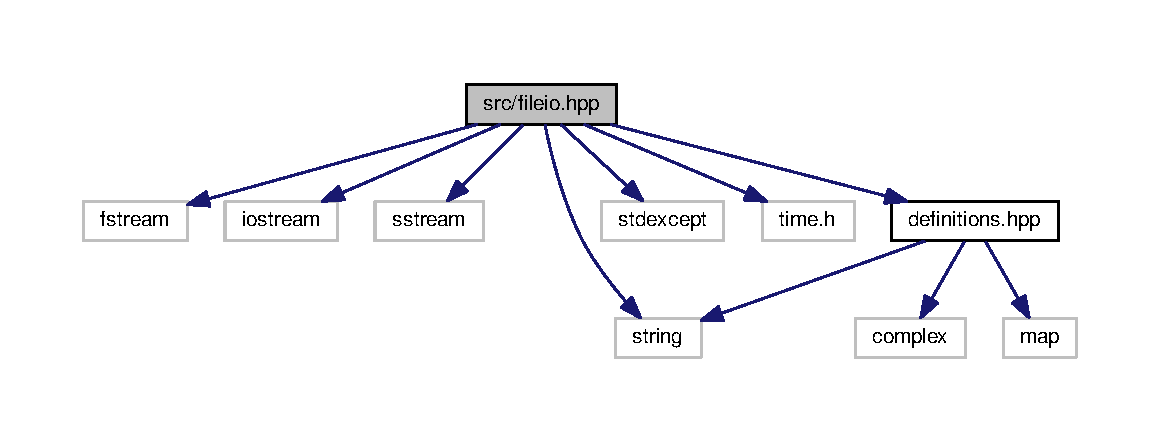
\includegraphics[width=350pt]{fileio_8hpp__incl}
\end{center}
\end{figure}
This graph shows which files directly or indirectly include this file\+:
\nopagebreak
\begin{figure}[H]
\begin{center}
\leavevmode
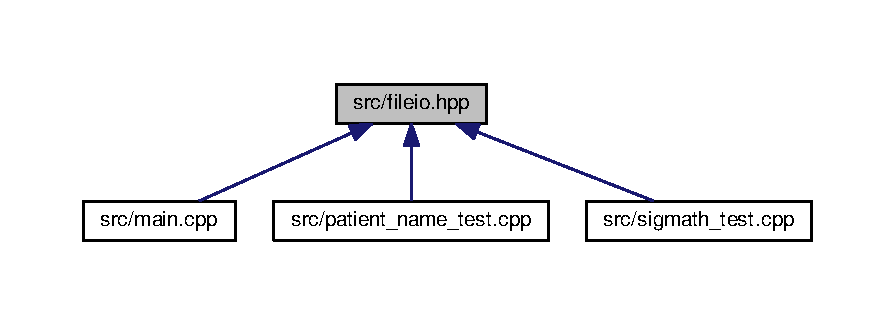
\includegraphics[width=350pt]{fileio_8hpp__dep__incl}
\end{center}
\end{figure}
\subsection*{Namespaces}
\begin{DoxyCompactItemize}
\item 
 \hyperlink{namespaceavda}{avda}
\end{DoxyCompactItemize}
\subsection*{Functions}
\begin{DoxyCompactItemize}
\item 
std\+::string \hyperlink{namespaceavda_ae20728e7e8ae50bf2f74849e538841ea}{avda\+::\+Patient\+Name} ()
\item 
std\+::map$<$ Side, \hyperlink{structDataParams}{Data\+Params} $>$ \hyperlink{namespaceavda_a46dc980b65ddfc24749ce25c1290e158}{avda\+::\+Read\+Params} (auto filename)
\item 
void \hyperlink{namespaceavda_aba04a08b41833ced32ec803d55a63bee}{avda\+::\+Write\+Params} (std\+::map$<$ Side, \hyperlink{structDataParams}{Data\+Params} $>$ my\+Map, auto filename)
\end{DoxyCompactItemize}
\subsection*{Variables}
\begin{DoxyCompactItemize}
\item 
const std\+::string \hyperlink{namespaceavda_ac568a0872c2c176d874b8b12f67f43ea}{avda\+::\+C\+S\+V\+\_\+\+H\+E\+A\+D\+E\+R} = \char`\"{}Time,Side,Frequency,Noise Level\char`\"{}
\item 
const std\+::string \hyperlink{namespaceavda_a8ee73ec0cb55d4a13e89949764dce89d}{avda\+::\+P\+A\+T\+I\+E\+N\+T\+\_\+\+P\+A\+T\+H} = \char`\"{}/home/pi/patients/\char`\"{}
\end{DoxyCompactItemize}


\subsection{Detailed Description}
contains functions related to the file I/\+O use in this program 

\begin{DoxyAuthor}{Author}
Samuel Andrew Wisner, \href{mailto:awisner94@gmail.com}{\tt awisner94@gmail.\+com} 

Nicholas K. Nolan 
\end{DoxyAuthor}
\begin{DoxyRefDesc}{Bug}
\item[\hyperlink{bug__bug000001}{Bug}]file is overly complicated and much more bug-\/prone \end{DoxyRefDesc}


Definition in file \hyperlink{fileio_8hpp_source}{fileio.\+hpp}.


\hypertarget{fileio_8hpp_source}{\section{fileio.\+hpp}
\label{fileio_8hpp_source}\index{src/fileio.\+hpp@{src/fileio.\+hpp}}
}

\begin{DoxyCode}
00001 
00009 \textcolor{preprocessor}{#ifndef fileio\_H}
00010 \textcolor{preprocessor}{#define fileio\_H}
00011 
00012 \textcolor{preprocessor}{#include <fstream>}
00013 \textcolor{preprocessor}{#include <iostream>}
00014 \textcolor{preprocessor}{#include <sstream>}
00015 \textcolor{preprocessor}{#include <string>}
00016 \textcolor{preprocessor}{#include <stdexcept>}
00017 \textcolor{preprocessor}{#include <time.h>}
00018 
00019 \textcolor{preprocessor}{#include "\hyperlink{definitions_8hpp}{definitions.hpp}"}
00020 
00021 \textcolor{keyword}{namespace }\hyperlink{namespaceavda}{avda} \{
\hypertarget{fileio_8hpp_source_l00025}{}\hyperlink{namespaceavda_ac568a0872c2c176d874b8b12f67f43ea}{00025}     \textcolor{keyword}{const} std::string \hyperlink{namespaceavda_ac568a0872c2c176d874b8b12f67f43ea}{CSV\_HEADER} = \textcolor{stringliteral}{"Time,Side,Frequency,Noise Level"};
00026 
\hypertarget{fileio_8hpp_source_l00030}{}\hyperlink{namespaceavda_a8ee73ec0cb55d4a13e89949764dce89d}{00030}     \textcolor{keyword}{const} std::string \hyperlink{namespaceavda_a8ee73ec0cb55d4a13e89949764dce89d}{PATIENT\_PATH} = \textcolor{stringliteral}{"/home/pi/patients/"};
00031 
\hypertarget{fileio_8hpp_source_l00043}{}\hyperlink{namespaceavda_ae20728e7e8ae50bf2f74849e538841ea}{00043}     std::string \hyperlink{namespaceavda_ae20728e7e8ae50bf2f74849e538841ea}{PatientName}() \{
00044         std::string fname = \textcolor{stringliteral}{""};
00045         std::string mname = \textcolor{stringliteral}{""};
00046         std::string lname = \textcolor{stringliteral}{""};
00047         std::string patfil = \textcolor{stringliteral}{""};
00048         std::string patientname = \textcolor{stringliteral}{""};
00049         \hyperlink{definitions_8hpp_a1134b580f8da4de94ca6b1de4d37975e}{uint32} track1 = 0;
00050         \hyperlink{definitions_8hpp_a1134b580f8da4de94ca6b1de4d37975e}{uint32} track2 = 0;
00051         \hyperlink{definitions_8hpp_a1134b580f8da4de94ca6b1de4d37975e}{uint32} track3 = 0;
00052 
00053         \textcolor{keywordflow}{do} \{
00054             std::cout << \textcolor{stringliteral}{"Please enter the patients name."} << std::endl;
00055             std::cout << \textcolor{stringliteral}{"First name: "};
00056             std::cin >> fname;
00057             std::cout << \textcolor{stringliteral}{"Middle name: "};
00058             std::cin >> mname;
00059             std::cout << \textcolor{stringliteral}{"Last name: "};
00060             std::cin >> lname;
00061 
00062             \textcolor{comment}{// creates new std::string with path to patient file}
00063             patientname = PATIENT\_PATH + lname + \textcolor{stringliteral}{", "} + fname
00064                 + \textcolor{stringliteral}{" "} + mname + \textcolor{stringliteral}{".csv"};
00065 
00066             \textcolor{comment}{// prints out patientname. shows user the path to the patient file}
00067             \textcolor{comment}{//std::cout << patientname << std::endl << std::endl;}
00068             std::ifstream file(patientname.c\_str());
00069 
00070             \textcolor{keywordflow}{if} (file.good()) \{
00071                 track1 = 1;
00072             \}
00073 
00074             \textcolor{comment}{/*}
00075 \textcolor{comment}{             * Compares patientname to existing files and lets user know}
00076 \textcolor{comment}{             * if the file does not exist.}
00077 \textcolor{comment}{             */}
00078             \textcolor{keywordflow}{else} \textcolor{keywordflow}{if} (!file.good()) \{
00079                 \textcolor{comment}{/* }
00080 \textcolor{comment}{                 * Do while statement to continue asking user about the file}
00081 \textcolor{comment}{                 * if their input is not acceptable}
00082 \textcolor{comment}{                 */} 
00083                 \textcolor{keywordflow}{do} \{
00084                     std::cout << \textcolor{stringliteral}{"Patient file does not exist, would you like "}
00085                         \textcolor{stringliteral}{"to create file or re-enter their name?"} << std::endl;
00086                     std::cout << \textcolor{stringliteral}{"  *Type 'create' and press enter key "}
00087                         \textcolor{stringliteral}{"to create the patient file."} << std::endl;
00088                     std::cout << \textcolor{stringliteral}{"  *Type 'reenter' and press enter key "}
00089                         \textcolor{stringliteral}{"to re-enter the patients name."} << std::endl;
00090                     std::cout << std::endl;
00091                     std::cin >> patfil;
00092 
00093                     \textcolor{comment}{/* }
00094 \textcolor{comment}{                     * patfil equals create, track1 and 2 will increase}
00095 \textcolor{comment}{                     * escaping both do while loops}
00096 \textcolor{comment}{                     */}
00097                     \textcolor{keywordflow}{if}(patfil == \textcolor{stringliteral}{"create"}) \{
00098                         std::ofstream createfile(patientname.c\_str());
00099                         track1 = 1;
00100                         track2 = 1;
00101                         track3 = 1;
00102                         createfile << CSV\_HEADER << std::endl;
00103                         createfile.flush();
00104                         createfile.close();
00105                     \}
00106 
00107                     \textcolor{comment}{/*}
00108 \textcolor{comment}{                     *patfil equals renter, track1 will remain zero allowing}
00109 \textcolor{comment}{                     *user to reenter the patient name.}
00110 \textcolor{comment}{                     */}
00111                     \textcolor{keywordflow}{else} \textcolor{keywordflow}{if}(patfil == \textcolor{stringliteral}{"reenter"}) \{
00112                         track1 = 0;
00113                         track2 = 1;
00114                     \}
00115 
00116                     \textcolor{comment}{/*}
00117 \textcolor{comment}{                     *The users input was neither create or reenter. User}
00118 \textcolor{comment}{                     *must enter patient name again.}
00119 \textcolor{comment}{                     */}
00120                     \textcolor{keywordflow}{else} \{
00121                         std::cout << std::endl;
00122                         std::cout << \textcolor{stringliteral}{"Your input is not acceptable."} << std::endl;
00123                         std::cout << std::endl;
00124                     \}
00125                 \}\textcolor{keywordflow}{while}(track2 == 0);
00126             \}
00127         \} \textcolor{keywordflow}{while} (track1 == 0);
00128 
00129         \textcolor{keywordflow}{return} patientname; \textcolor{comment}{//returns the path to the patient file}
00130     \}
00131 
\hypertarget{fileio_8hpp_source_l00141}{}\hyperlink{namespaceavda_a46dc980b65ddfc24749ce25c1290e158}{00141}     std::map<Side, DataParams> \hyperlink{namespaceavda_a46dc980b65ddfc24749ce25c1290e158}{ReadParams}(\textcolor{keyword}{auto} filename) \{
00142         std::map<Side, DataParams> myMap;
00143         \hyperlink{structDataParams}{DataParams} leftparams;
00144         \hyperlink{structDataParams}{DataParams} rightparams;
00145 
00146         std::ifstream file(filename.c\_str());
00147         std::string leftline;
00148         std::string rightline;
00149         std::string leftsearch = \textcolor{stringliteral}{"Left"};
00150         std::string rightsearch = \textcolor{stringliteral}{"Right"};
00151         std::string paramstring;
00152         std::string lfreqstr;
00153         std::string lnoisestr;
00154         std::string rfreqstr;
00155         std::string rnoisestr;
00156         \hyperlink{definitions_8hpp_a1134b580f8da4de94ca6b1de4d37975e}{uint32} lcnt = 0;
00157         \hyperlink{definitions_8hpp_a1134b580f8da4de94ca6b1de4d37975e}{uint32} rcnt = 0;
00158         \hyperlink{definitions_8hpp_aacdc525d6f7bddb3ae95d5c311bd06a1}{float32} lfreqval;
00159         \hyperlink{definitions_8hpp_aacdc525d6f7bddb3ae95d5c311bd06a1}{float32} lnoiseval;
00160         \hyperlink{definitions_8hpp_aacdc525d6f7bddb3ae95d5c311bd06a1}{float32} rfreqval;
00161         \hyperlink{definitions_8hpp_aacdc525d6f7bddb3ae95d5c311bd06a1}{float32} rnoiseval;
00162 
00163         \textcolor{comment}{/*}
00164 \textcolor{comment}{         * if statement which uses ifstream function to open patient file }
00165 \textcolor{comment}{         * filename)}
00166 \textcolor{comment}{         */}
00167         \textcolor{keywordflow}{if}(file.is\_open()) \{
00168             \textcolor{comment}{/*}
00169 \textcolor{comment}{             * While statement to find the first Left line and save to }
00170 \textcolor{comment}{             *leftline as string.}
00171 \textcolor{comment}{             */}
00172             \textcolor{keywordflow}{while} (getline(file, leftline)) \{
00173                 \textcolor{keywordflow}{if}(leftline.find(leftsearch, 0) != std::string::npos) \{
00174                     \textcolor{keywordflow}{break};
00175                 \}
00176 
00177             \}
00178 
00179             \textcolor{comment}{/*}
00180 \textcolor{comment}{             * While statement to find first right line and save to rightline}
00181 \textcolor{comment}{             * as string.}
00182 \textcolor{comment}{             */}
00183             \textcolor{keywordflow}{while} (getline(file,rightline)) \{
00184                 \textcolor{keywordflow}{if}(rightline.find(rightsearch, 0) != std::string::npos) \{
00185                     \textcolor{keywordflow}{break};
00186                 \}
00187             \}
00188 
00189             \textcolor{comment}{// Code to break leftline and rightline into its parts}
00190             std::stringstream lss(leftline);
00191             std::stringstream rss(rightline);
00192 
00193             \textcolor{keywordflow}{while}(getline(lss,paramstring, \textcolor{charliteral}{','})) \{
00194                 lcnt++;
00195 
00196                 \textcolor{keywordflow}{if}(lcnt == 3) \{
00197                     lfreqstr = paramstring;
00198                 \}
00199 
00200                 \textcolor{keywordflow}{else} \textcolor{keywordflow}{if}(lcnt == 4) \{
00201                     lnoisestr = paramstring;
00202                 \}
00203             \}
00204 
00205             \textcolor{keywordflow}{while}(getline(rss,paramstring, \textcolor{charliteral}{','})) \{
00206                 rcnt++;
00207 
00208                 \textcolor{keywordflow}{if}(rcnt == 3) \{
00209                     rfreqstr = paramstring;
00210                 \}
00211 
00212                 \textcolor{keywordflow}{else} \textcolor{keywordflow}{if}(rcnt == 4) \{
00213                     rnoisestr = paramstring;
00214                 \}
00215             \}
00216 
00217             \textcolor{comment}{/*}
00218 \textcolor{comment}{             * Statement to convert lfreq, lnoise, rfreq, and rnoise from}
00219 \textcolor{comment}{             * strings to floats.}
00220 \textcolor{comment}{             * */}
00221             lfreqval = atof(lfreqstr.c\_str());
00222             lnoiseval = atof(lnoisestr.c\_str());
00223             rfreqval = atof(rfreqstr.c\_str());
00224             rnoiseval = atof(rnoisestr.c\_str());
00225 
00226             file.close();
00227         \}
00228 
00229         \textcolor{keywordflow}{else} \{
00230             \textcolor{keywordflow}{throw} std::runtime\_error(\textcolor{stringliteral}{"The patient file could not be opened."});
00231         \}
00232 
00233         leftparams.\hyperlink{structDataParams_a12566e017407647bc8287d62554ad3fb}{freq} = lfreqval;
00234         leftparams.\hyperlink{structDataParams_a4efd1d2231c6fa7c878c9d5e1650738f}{noise} = lnoiseval;
00235         rightparams.\hyperlink{structDataParams_a12566e017407647bc8287d62554ad3fb}{freq} = rfreqval;
00236         rightparams.\hyperlink{structDataParams_a4efd1d2231c6fa7c878c9d5e1650738f}{noise} = rnoiseval;
00237 
00238         myMap[\hyperlink{namespaceavda_af723e82f0d3d45fda6fdc01f6a492786a945d5e233cf7d6240f6b783b36a374ff}{Side::Left}] = leftparams;
00239         myMap[\hyperlink{namespaceavda_af723e82f0d3d45fda6fdc01f6a492786a92b09c7c48c520c3c55e497875da437c}{Side::Right}] = rightparams;
00240 
00241         \textcolor{keywordflow}{return} myMap;
00242     \}
00243 
\hypertarget{fileio_8hpp_source_l00251}{}\hyperlink{namespaceavda_aba04a08b41833ced32ec803d55a63bee}{00251}     \textcolor{keywordtype}{void} \hyperlink{namespaceavda_aba04a08b41833ced32ec803d55a63bee}{WriteParams}(std::map<Side, DataParams> myMap, \textcolor{keyword}{auto} filename) \{
00252         \textcolor{keywordtype}{char} temp[80];
00253         std::ofstream file(filename.c\_str(),
00254                 std::ofstream::out | std::ofstream::app);
00255 
00256         \textcolor{comment}{//Gives pointer measurementtime a data type of time\_t.}
00257         time\_t measurementtime;
00258         time(&measurementtime); \textcolor{comment}{//Gets the current time.}
00259         strftime(temp, 80, \textcolor{stringliteral}{"%c"}, localtime(&measurementtime));
00260         std::string fTime = std::string(temp);
00261 
00262         \textcolor{comment}{//if statement to print the Left side parameters to the patient file.}
00263         \textcolor{keywordflow}{if}(file.is\_open()) \{
00264             file << fTime + \textcolor{stringliteral}{","} + \textcolor{stringliteral}{"Left"} + \textcolor{stringliteral}{","}
00265                 + std::to\_string(myMap[\hyperlink{namespaceavda_af723e82f0d3d45fda6fdc01f6a492786a945d5e233cf7d6240f6b783b36a374ff}{Side::Left}].freq) 
00266                 + \textcolor{stringliteral}{", "} + std::to\_string(myMap[\hyperlink{namespaceavda_af723e82f0d3d45fda6fdc01f6a492786a945d5e233cf7d6240f6b783b36a374ff}{Side::Left}].noise) << std::endl;
00267         \}
00268 
00269         \textcolor{comment}{//if statement to print the Right side parameters to the patient file.}
00270         \textcolor{keywordflow}{if}(file.is\_open()) \{
00271             file << fTime + \textcolor{stringliteral}{","} + \textcolor{stringliteral}{"Right"} + \textcolor{stringliteral}{","}
00272                 + std::to\_string(myMap[\hyperlink{namespaceavda_af723e82f0d3d45fda6fdc01f6a492786a92b09c7c48c520c3c55e497875da437c}{Side::Right}].freq) 
00273                 + \textcolor{stringliteral}{", "} + std::to\_string(myMap[\hyperlink{namespaceavda_af723e82f0d3d45fda6fdc01f6a492786a92b09c7c48c520c3c55e497875da437c}{Side::Right}].noise) << std::endl;
00274         \}
00275 
00276         \textcolor{keywordflow}{else} \{
00277             std::cout << \textcolor{stringliteral}{"Patient file can not be opened!"} << std::endl;
00278         \}
00279 
00280         file.close();
00281     \}
00282 \}
00283 
00284 \textcolor{preprocessor}{#endif}
\end{DoxyCode}

\hypertarget{main_8cpp}{\section{src/main.cpp File Reference}
\label{main_8cpp}\index{src/main.\+cpp@{src/main.\+cpp}}
}
{\ttfamily \#include $<$array$>$}\\*
{\ttfamily \#include $<$cstdlib$>$}\\*
{\ttfamily \#include $<$iostream$>$}\\*
{\ttfamily \#include $<$map$>$}\\*
{\ttfamily \#include $<$pthread.\+h$>$}\\*
{\ttfamily \#include $<$string$>$}\\*
{\ttfamily \#include $<$unistd.\+h$>$}\\*
{\ttfamily \#include \char`\"{}definitions.\+hpp\char`\"{}}\\*
{\ttfamily \#include \char`\"{}fileio.\+hpp\char`\"{}}\\*
{\ttfamily \#include \char`\"{}process.\+hpp\char`\"{}}\\*
Include dependency graph for main.\+cpp\+:
\nopagebreak
\begin{figure}[H]
\begin{center}
\leavevmode
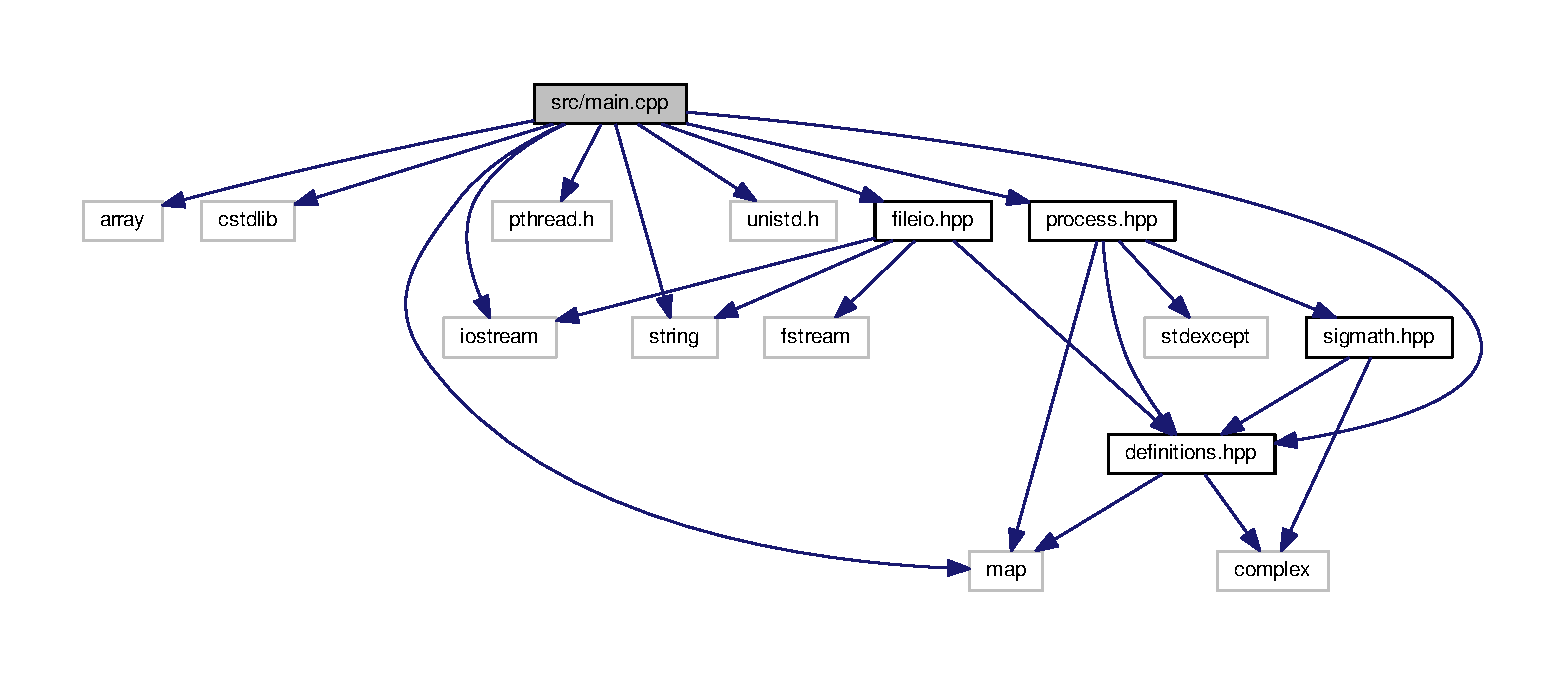
\includegraphics[width=350pt]{main_8cpp__incl}
\end{center}
\end{figure}
\subsection*{Functions}
\begin{DoxyCompactItemize}
\item 
int \hyperlink{main_8cpp_a3c04138a5bfe5d72780bb7e82a18e627}{main} (int argc, char $\ast$$\ast$argv)
\end{DoxyCompactItemize}


\subsection{Function Documentation}
\hypertarget{main_8cpp_a3c04138a5bfe5d72780bb7e82a18e627}{\index{main.\+cpp@{main.\+cpp}!main@{main}}
\index{main@{main}!main.\+cpp@{main.\+cpp}}
\subsubsection[{main}]{\setlength{\rightskip}{0pt plus 5cm}int main (
\begin{DoxyParamCaption}
\item[{int}]{argc, }
\item[{char $\ast$$\ast$}]{argv}
\end{DoxyParamCaption}
)}}\label{main_8cpp_a3c04138a5bfe5d72780bb7e82a18e627}
The main program for this progject. It will detect vasospasms over a period of days. 

Definition at line \hyperlink{main_8cpp_source_l00026}{26} of file \hyperlink{main_8cpp_source}{main.\+cpp}.



Here is the call graph for this function\+:
\nopagebreak
\begin{figure}[H]
\begin{center}
\leavevmode
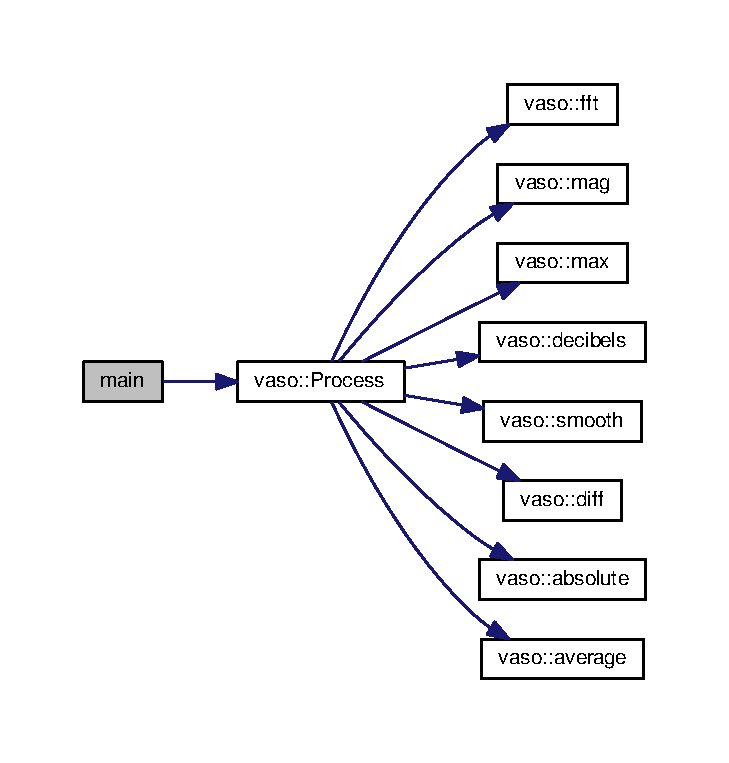
\includegraphics[width=350pt]{main_8cpp_a3c04138a5bfe5d72780bb7e82a18e627_cgraph}
\end{center}
\end{figure}



\hypertarget{main_8cpp_source}{\section{main.\+cpp}
\label{main_8cpp_source}\index{src/main.\+cpp@{src/main.\+cpp}}
}

\begin{DoxyCode}
00001 
00010 \textcolor{preprocessor}{#include <array>}
00011 \textcolor{preprocessor}{#include <cstdio>}
00012 \textcolor{preprocessor}{#include <cstdlib>}
00013 \textcolor{preprocessor}{#include <fcntl.h>}
00014 \textcolor{preprocessor}{#include <iostream>}
00015 \textcolor{preprocessor}{#include <map>}
00016 \textcolor{preprocessor}{#include <pthread.h>}
00017 \textcolor{preprocessor}{#include <string>}
00018 \textcolor{preprocessor}{#include <unistd.h>}
00019 
00020 \textcolor{preprocessor}{#include "\hyperlink{definitions_8hpp}{definitions.hpp}"}
00021 \textcolor{preprocessor}{#include "\hyperlink{fileio_8hpp}{fileio.hpp}"}
00022 \textcolor{preprocessor}{#include "\hyperlink{process_8hpp}{process.hpp}"}
00023 
00024 \textcolor{keyword}{using namespace }\hyperlink{namespacestd}{std};
00025 \textcolor{keyword}{using namespace }\hyperlink{namespaceavda}{avda};
00026 
\hypertarget{main_8cpp_source_l00031}{}\hyperlink{main_8cpp_a3c04138a5bfe5d72780bb7e82a18e627}{00031} \textcolor{keywordtype}{int} \hyperlink{main_8cpp_a3c04138a5bfe5d72780bb7e82a18e627}{main}(\textcolor{keywordtype}{int} argc, \textcolor{keywordtype}{char}** argv) \{
00032     \textcolor{comment}{// Recorded audio buffer}
00033     \hyperlink{definitions_8hpp_aacdc525d6f7bddb3ae95d5c311bd06a1}{float32}* buffer = (\hyperlink{definitions_8hpp_aacdc525d6f7bddb3ae95d5c311bd06a1}{float32}*)std::malloc(\hyperlink{definitions_8hpp_aca681ed285767aaa2353bf3b42dd60ed}{BUFFER\_SIZE});
00034     \textcolor{keywordtype}{bool} cont = \textcolor{keyword}{true};  \textcolor{comment}{// whether to continue in the recording loop}
00035     \hyperlink{structDataParams}{DataParams} params[\hyperlink{definitions_8hpp_a2fd18fd694a2918f7d73eba821fd10b2}{REC\_COUNT}];  \textcolor{comment}{// holds DataParam's from recordings}
00036     \textcolor{keywordtype}{string} filename = \hyperlink{namespaceavda_ae20728e7e8ae50bf2f74849e538841ea}{PatientName}();  \textcolor{comment}{// generate name for patient's file}
00037     map<Side, DataParams> results;  \textcolor{comment}{// parameters by side}
00038 
00039     \textcolor{comment}{// arecord command}
00040     \textcolor{keyword}{const} \textcolor{keywordtype}{string} recCommand = string(\textcolor{stringliteral}{"arecord -t raw -d "})
00041         + to\_string(\hyperlink{definitions_8hpp_ada7a88c013312e76596a2000cc8277fb}{DURATION}) + string(\textcolor{stringliteral}{" -D plughw:1,0 -f FLOAT -q -r "})
00042         + to\_string(\hyperlink{definitions_8hpp_a8ace559345ecba7978591ac2ef22aea4}{SAMPLE\_FREQ}) + string(\textcolor{stringliteral}{" "}) + \hyperlink{definitions_8hpp_a88f32e97c41b89ff0705d0a0b8566b41}{TEMP\_FILE};
00043 
00044     \textcolor{comment}{// Recording}
00045     \textcolor{keywordflow}{while}(cont) \{
00046         \textcolor{keywordflow}{for}(\hyperlink{definitions_8hpp_adde6aaee8457bee49c2a92621fe22b79}{uint8} i = 0; i < \hyperlink{definitions_8hpp_a2fd18fd694a2918f7d73eba821fd10b2}{REC\_COUNT}; i++) \{
00047             \textcolor{comment}{// prompt}
00048             cout << \textcolor{stringliteral}{"Press [ ENTER ] to begin analysis for the "}
00049                 << (i < REC\_COUNT / 2 ? \textcolor{stringliteral}{"left"} : \textcolor{stringliteral}{"right"}) << \textcolor{stringliteral}{" side, depth #"}
00050                 << (((i >= REC\_COUNT / 2) ? (i - REC\_COUNT / 2) : i) + 1)
00051                 << \textcolor{stringliteral}{" "};
00052             getchar();  \textcolor{comment}{// wait for ENTER to be pressed}
00053             cout << \textcolor{stringliteral}{"Analyzing..."} << endl;
00054 
00055             system(recCommand.c\_str());
00056             usleep(\hyperlink{definitions_8hpp_ada7a88c013312e76596a2000cc8277fb}{DURATION}*1000000 + 1500000);  \textcolor{comment}{// sleep DURATION + 1.5 seconds}
00057 
00058             \textcolor{keywordtype}{int} file = open(\hyperlink{definitions_8hpp_a88f32e97c41b89ff0705d0a0b8566b41}{TEMP\_FILE}.c\_str(), O\_RDONLY);  \textcolor{comment}{// open temp file}
00059             \textcolor{keywordtype}{int} retRead = read(file, buffer, \hyperlink{definitions_8hpp_aca681ed285767aaa2353bf3b42dd60ed}{BUFFER\_SIZE});  \textcolor{comment}{// copy to buffer}
00060             close(file);  \textcolor{comment}{// close temp file}
00061             \textcolor{keyword}{remove}(\hyperlink{definitions_8hpp_a88f32e97c41b89ff0705d0a0b8566b41}{TEMP\_FILE}.c\_str());  \textcolor{comment}{// delete temp file}
00062 
00063             \textcolor{comment}{// if something goes wrong reading the temp file, program exits}
00064             \textcolor{keywordflow}{if}(file < 0 || retRead < \hyperlink{definitions_8hpp_aca681ed285767aaa2353bf3b42dd60ed}{BUFFER\_SIZE}) \{
00065                 cerr << \textcolor{stringliteral}{"An error occurred reading the doppler audio! "}
00066                     \textcolor{stringliteral}{"The program will now exit."} << endl;
00067                 \textcolor{keywordflow}{return} \hyperlink{definitions_8hpp_a876fcacb67d51738e846a3312dc08fbb}{ERROR};
00068             \}
00069 
00070             \textcolor{comment}{// process and store parameters}
00071             params[i] = \hyperlink{namespaceavda_a5196cce27286d08ca144a460caee7839}{process}(buffer, \hyperlink{definitions_8hpp_ad3af99f5e7cbf2af51be580e91faa934}{SAMPLE\_COUNT}, 
      \hyperlink{definitions_8hpp_a8ace559345ecba7978591ac2ef22aea4}{SAMPLE\_FREQ});
00072             cout << \textcolor{stringliteral}{"The analysis is complete."} << endl << endl;
00073         \}
00074 
00075         \textcolor{comment}{// calculate averaged parameters}
00076         results[Side::Left] = \hyperlink{namespaceavda_a2a830f24a59aa2538ea82f6e000cce61}{average}(params, REC\_COUNT / 2);
00077         results[Side::Right] = \hyperlink{namespaceavda_a2a830f24a59aa2538ea82f6e000cce61}{average}(&params[REC\_COUNT / 2], REC\_COUNT / 2);
00078 
00079         cout << \textcolor{stringliteral}{"Analysis is complete."} << endl << endl;
00080 
00081         \textcolor{comment}{// print averaged side analysis}
00082         \textcolor{keywordflow}{for}(\textcolor{keywordtype}{int} i = 0; i < 2; i++) \{
00083             \hyperlink{namespaceavda_af723e82f0d3d45fda6fdc01f6a492786}{Side} side = (\hyperlink{namespaceavda_af723e82f0d3d45fda6fdc01f6a492786}{Side})i;
00084             cout << (side == Side::Left ? \textcolor{stringliteral}{"[LEFT]"} : \textcolor{stringliteral}{"[RIGHT]"}) << endl;
00085             cout << \textcolor{stringliteral}{"Drop-off frequency: "} << (\hyperlink{definitions_8hpp_a05f6b0ae8f6a6e135b0e290c25fe0e4e}{uint16})(results[side].freq + 0.5)
00086                 << \textcolor{stringliteral}{" Hz"} << endl;
00087             cout << \textcolor{stringliteral}{"Average relative noiseband power: "}
00088                 << (\hyperlink{definitions_8hpp_a74df79fde3c518e55b29ce6360a9c76e}{sint16})(results[side].noise - 0.5) << \textcolor{stringliteral}{" dB"} << endl <<endl;
00089         \}
00090 
00091         cont = results[Side::Left].freq > \hyperlink{definitions_8hpp_ab506614aee9be52f401d8d573a8d172c}{MAX\_DROP\_FREQ}
00092             || results[Side::Right].freq > \hyperlink{definitions_8hpp_ab506614aee9be52f401d8d573a8d172c}{MAX\_DROP\_FREQ};
00093 
00094         \textcolor{keywordflow}{if}(cont) \{
00095             cout << \textcolor{stringliteral}{"An error in aquisition of the doppler audio has occurred! "}
00096                 \textcolor{stringliteral}{"Ensure the connection from the doppler machine to this device "}
00097                 \textcolor{stringliteral}{"is secure and the connection uninterruptable."} << endl << endl;
00098         \}
00099     \}
00100 
00101     free(buffer);  \textcolor{comment}{// free buffer to prevent memory leak}
00102     \hyperlink{namespaceavda_aba04a08b41833ced32ec803d55a63bee}{WriteParams}(results, filename);
00103 
00104     \textcolor{comment}{// examine likelihood of avdaspasm}
00105     \textcolor{keywordflow}{try} \{
00106         map<Side, DataParams> baseParams = \hyperlink{namespaceavda_a46dc980b65ddfc24749ce25c1290e158}{ReadParams}(filename);
00107         map<Side, bool> comparison;
00108 
00109         \textcolor{keywordflow}{for}(\hyperlink{definitions_8hpp_adde6aaee8457bee49c2a92621fe22b79}{uint8} i = 0; i < 2; i++) \{
00110             \hyperlink{namespaceavda_af723e82f0d3d45fda6fdc01f6a492786}{Side} side = (\hyperlink{namespaceavda_af723e82f0d3d45fda6fdc01f6a492786}{Side})i;
00111             \textcolor{keywordtype}{float} comp = (results[side].freq - baseParams[side].freq) 
00112                 * (baseParams[side].noise - results[side].noise);
00113             comparison[side] = comp > \hyperlink{definitions_8hpp_aa15adfcc96559f1b86210d217edd3afc}{DET\_THRESH};
00114         \}
00115 
00116         \textcolor{keywordtype}{string} which;
00117 
00118         \textcolor{keywordflow}{if}(comparison[Side::Left] && !comparison[Side::Right]) \{
00119             which = \textcolor{stringliteral}{"The left"};
00120         \} \textcolor{keywordflow}{else} \textcolor{keywordflow}{if}(!comparison[Side::Left] && comparison[Side::Right]) \{
00121             which = \textcolor{stringliteral}{"The right"};
00122         \} \textcolor{keywordflow}{else} \textcolor{keywordflow}{if} (comparison[Side::Left] && comparison[Side::Right]) \{
00123             which = \textcolor{stringliteral}{"Both"};
00124         \} \textcolor{keywordflow}{else} \{
00125             which = \textcolor{stringliteral}{"Neither"};
00126         \}
00127 
00128         cout << which << \textcolor{stringliteral}{" side seems to show evidence of a vasospasm."} << endl;
00129     \} \textcolor{keywordflow}{catch}(runtime\_error ex) \{
00130         cout << \textcolor{stringliteral}{"These values will be stored as the baseline parameters to "}
00131             \textcolor{stringliteral}{"which all future parameters are compared."} << endl;
00132     \}
00133 \}
\end{DoxyCode}

\hypertarget{patient__name__test_8cpp}{\section{src/patient\+\_\+name\+\_\+test.cpp File Reference}
\label{patient__name__test_8cpp}\index{src/patient\+\_\+name\+\_\+test.\+cpp@{src/patient\+\_\+name\+\_\+test.\+cpp}}
}
{\ttfamily \#include $<$string$>$}\\*
{\ttfamily \#include \char`\"{}definitions.\+hpp\char`\"{}}\\*
{\ttfamily \#include \char`\"{}fileio.\+hpp\char`\"{}}\\*
{\ttfamily \#include \char`\"{}process.\+hpp\char`\"{}}\\*
Include dependency graph for patient\+\_\+name\+\_\+test.\+cpp\+:
\nopagebreak
\begin{figure}[H]
\begin{center}
\leavevmode
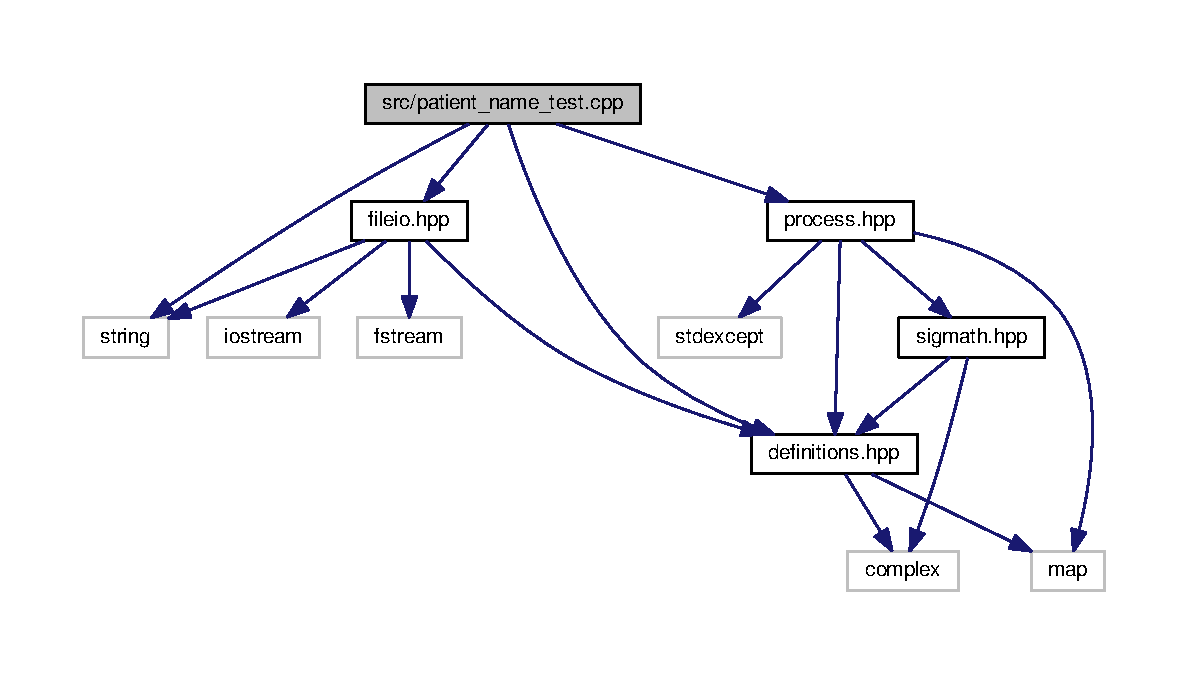
\includegraphics[width=350pt]{patient__name__test_8cpp__incl}
\end{center}
\end{figure}
\subsection*{Functions}
\begin{DoxyCompactItemize}
\item 
int \hyperlink{patient__name__test_8cpp_a3c04138a5bfe5d72780bb7e82a18e627}{main} (int argc, char $\ast$$\ast$argv)
\end{DoxyCompactItemize}


\subsection{Function Documentation}
\hypertarget{patient__name__test_8cpp_a3c04138a5bfe5d72780bb7e82a18e627}{\index{patient\+\_\+name\+\_\+test.\+cpp@{patient\+\_\+name\+\_\+test.\+cpp}!main@{main}}
\index{main@{main}!patient\+\_\+name\+\_\+test.\+cpp@{patient\+\_\+name\+\_\+test.\+cpp}}
\subsubsection[{main}]{\setlength{\rightskip}{0pt plus 5cm}int main (
\begin{DoxyParamCaption}
\item[{int}]{argc, }
\item[{char $\ast$$\ast$}]{argv}
\end{DoxyParamCaption}
)}}\label{patient__name__test_8cpp_a3c04138a5bfe5d72780bb7e82a18e627}


Definition at line \hyperlink{patient__name__test_8cpp_source_l00020}{20} of file \hyperlink{patient__name__test_8cpp_source}{patient\+\_\+name\+\_\+test.\+cpp}.



Here is the call graph for this function\+:
\nopagebreak
\begin{figure}[H]
\begin{center}
\leavevmode
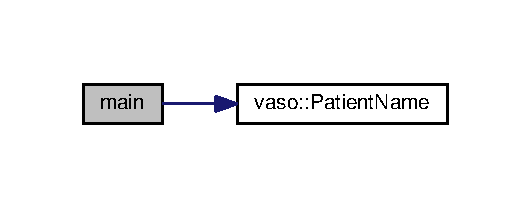
\includegraphics[width=255pt]{patient__name__test_8cpp_a3c04138a5bfe5d72780bb7e82a18e627_cgraph}
\end{center}
\end{figure}



\hypertarget{patient__name__test_8cpp_source}{\section{patient\+\_\+name\+\_\+test.\+cpp}
\label{patient__name__test_8cpp_source}\index{src/patient\+\_\+name\+\_\+test.\+cpp@{src/patient\+\_\+name\+\_\+test.\+cpp}}
}

\begin{DoxyCode}
00001 
00007 \textcolor{preprocessor}{#include <string>}
00008 
00009 \textcolor{preprocessor}{#include "\hyperlink{fileio_8hpp}{fileio.hpp}"}
00010 
00011 \textcolor{keyword}{using namespace }\hyperlink{namespacestd}{std};
00012 \textcolor{keyword}{using namespace }\hyperlink{namespaceavda}{avda};
00013 
\hypertarget{patient__name__test_8cpp_source_l00017}{}\hyperlink{patient__name__test_8cpp_a3c04138a5bfe5d72780bb7e82a18e627}{00017} \textcolor{keywordtype}{int} \hyperlink{patient__name__test_8cpp_a3c04138a5bfe5d72780bb7e82a18e627}{main}(\textcolor{keywordtype}{int} argc, \textcolor{keywordtype}{char}** argv) \{
00018     \textcolor{keywordtype}{string} filename = \hyperlink{namespaceavda_ae20728e7e8ae50bf2f74849e538841ea}{PatientName}();
00019     cout << filename;
00020 \}
\end{DoxyCode}

\hypertarget{process_8hpp}{\section{src/process.hpp File Reference}
\label{process_8hpp}\index{src/process.\+hpp@{src/process.\+hpp}}
}
{\ttfamily \#include $<$map$>$}\\*
{\ttfamily \#include $<$stdexcept$>$}\\*
{\ttfamily \#include \char`\"{}definitions.\+hpp\char`\"{}}\\*
{\ttfamily \#include \char`\"{}sigmath.\+hpp\char`\"{}}\\*
Include dependency graph for process.\+hpp\+:
\nopagebreak
\begin{figure}[H]
\begin{center}
\leavevmode
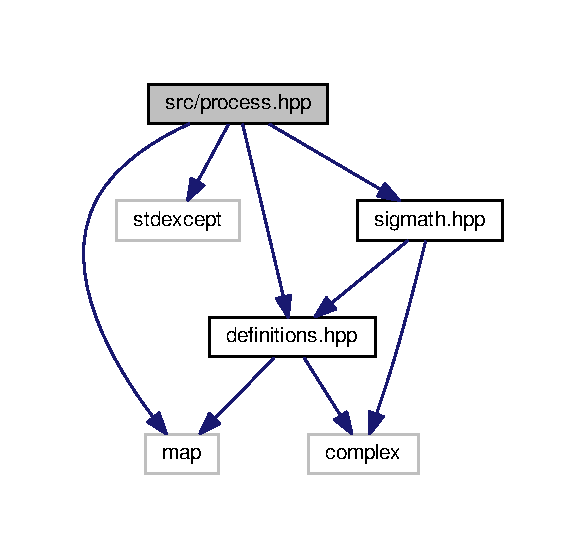
\includegraphics[width=281pt]{process_8hpp__incl}
\end{center}
\end{figure}
This graph shows which files directly or indirectly include this file\+:
\nopagebreak
\begin{figure}[H]
\begin{center}
\leavevmode
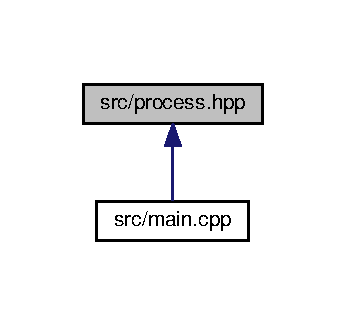
\includegraphics[width=350pt]{process_8hpp__dep__incl}
\end{center}
\end{figure}
\subsection*{Namespaces}
\begin{DoxyCompactItemize}
\item 
 \hyperlink{namespacevaso}{vaso}
\begin{DoxyCompactList}\small\item\em contains function()s related to the program's threaded processing of audio data \end{DoxyCompactList}\end{DoxyCompactItemize}
\subsection*{Functions}
\begin{DoxyCompactItemize}
\item 
std\+::map$<$ Side, \hyperlink{structDataParams}{Data\+Params} $>$ \hyperlink{namespacevaso_a0a7aa548b31b50c92be5b08bcb1df9a0}{vaso\+::\+Process} (\hyperlink{definitions_8hpp_aacdc525d6f7bddb3ae95d5c311bd06a1}{float32} $\ast$$\ast$data)
\item 
\hyperlink{structDataParams}{Data\+Params} \hyperlink{namespacevaso_a8136a2891983f7a41768330e018e3232}{vaso\+::process} (\hyperlink{definitions_8hpp_aacdc525d6f7bddb3ae95d5c311bd06a1}{float32} $\ast$data, \hyperlink{definitions_8hpp_a1134b580f8da4de94ca6b1de4d37975e}{uint32} size, \hyperlink{definitions_8hpp_aacdc525d6f7bddb3ae95d5c311bd06a1}{float32} sampling\+Rate)
\end{DoxyCompactItemize}

\hypertarget{process_8hpp_source}{\section{process.\+hpp}
\label{process_8hpp_source}\index{src/process.\+hpp@{src/process.\+hpp}}
}

\begin{DoxyCode}
00001 
00008 \textcolor{preprocessor}{#ifndef process\_H}
00009 \textcolor{preprocessor}{#define process\_H}
00010 
00011 \textcolor{preprocessor}{#include <map>}
00012 \textcolor{preprocessor}{#include <stdexcept>}
00013 
00014 \textcolor{preprocessor}{#include "\hyperlink{definitions_8hpp}{definitions.hpp}"}
00015 \textcolor{preprocessor}{#include "\hyperlink{sigmath_8hpp}{sigmath.hpp}"}
00016 
00017 \textcolor{keyword}{namespace }\hyperlink{namespaceavda}{avda} \{    
\hypertarget{process_8hpp_source_l00048}{}\hyperlink{namespaceavda_a5196cce27286d08ca144a460caee7839}{00048}     \hyperlink{structDataParams}{DataParams} \hyperlink{namespaceavda_a5196cce27286d08ca144a460caee7839}{process}(\hyperlink{definitions_8hpp_aacdc525d6f7bddb3ae95d5c311bd06a1}{float32}* data, \hyperlink{definitions_8hpp_a1134b580f8da4de94ca6b1de4d37975e}{uint32} size, 
      \hyperlink{definitions_8hpp_aacdc525d6f7bddb3ae95d5c311bd06a1}{float32} samplingRate) \{
00049         \textcolor{keywordflow}{if}((size & (size - 1) != 0) || size < 2) \{
00050             \textcolor{keywordflow}{throw} std::invalid\_argument(
00051                     \textcolor{stringliteral}{"The number of samples is not a power of two!"});
00052         \}
00053 
00054         \textcolor{comment}{// declare function-scoped variables}
00055         \hyperlink{definitions_8hpp_a1134b580f8da4de94ca6b1de4d37975e}{uint32} freqSize = size / 2;
00056         \hyperlink{definitions_8hpp_a960be6b6614c08090c16574dba10a421}{cfloat32}* cdata = (\hyperlink{definitions_8hpp_a960be6b6614c08090c16574dba10a421}{cfloat32}*)std::malloc(size * \textcolor{keyword}{sizeof}(
      \hyperlink{definitions_8hpp_a960be6b6614c08090c16574dba10a421}{cfloat32}));
00057         \hyperlink{definitions_8hpp_aacdc525d6f7bddb3ae95d5c311bd06a1}{float32}* fdata = (\hyperlink{definitions_8hpp_aacdc525d6f7bddb3ae95d5c311bd06a1}{float32}*)std::malloc(freqSize * \textcolor{keyword}{sizeof}(
      \hyperlink{definitions_8hpp_aacdc525d6f7bddb3ae95d5c311bd06a1}{float32}));
00058         \hyperlink{definitions_8hpp_aacdc525d6f7bddb3ae95d5c311bd06a1}{float32}* origdata = (\hyperlink{definitions_8hpp_aacdc525d6f7bddb3ae95d5c311bd06a1}{float32}*)std::malloc(freqSize * \textcolor{keyword}{sizeof}(
      \hyperlink{definitions_8hpp_aacdc525d6f7bddb3ae95d5c311bd06a1}{float32}));
00059 
00060         \textcolor{comment}{// convert data to complex numbers for fft()}
00061         \textcolor{keywordflow}{for}(\hyperlink{definitions_8hpp_a1134b580f8da4de94ca6b1de4d37975e}{uint32} i = 0; i < size; i++) \{
00062             cdata[i] = data[i];
00063         \}
00064     
00065         \textcolor{comment}{// find frequency spectrum in relative decibels}
00066         \hyperlink{namespaceavda_a33a1102422421212ac6b9387c896e864}{fft}(cdata, size);
00067         \hyperlink{namespaceavda_a213bd6384fc9a330e4db2cecdbcd73ee}{mag}(cdata, fdata, freqSize);
00068         \hyperlink{structMaximum}{Maximum} maximum = \hyperlink{namespaceavda_aa82021c3ee552773c060b1a39caf8aaa}{max}(fdata, freqSize);
00069 
00070         \textcolor{keywordflow}{for}(\hyperlink{definitions_8hpp_a1134b580f8da4de94ca6b1de4d37975e}{uint32} i = 0; i < freqSize; i++) \{
00071             fdata[i] /= maximum.\hyperlink{structMaximum_aa7e84cbf37b694670142670014366969}{value};
00072         \}
00073 
00074         \hyperlink{namespaceavda_a9c0b7f832eace3cbc9c5dddea2ecc9d5}{decibels}(fdata, freqSize);
00075 
00076         \textcolor{keywordflow}{for}(\hyperlink{definitions_8hpp_a1134b580f8da4de94ca6b1de4d37975e}{uint32} i = 0; i < freqSize; i++) \{
00077             origdata[i] = fdata[i];
00078         \}
00079 
00080         \textcolor{comment}{/*}
00081 \textcolor{comment}{         * Run spectrum values through moving-average filter to smooth the}
00082 \textcolor{comment}{         * curve and make it easier to determine the derivative.}
00083 \textcolor{comment}{         */}
00084         \hyperlink{namespaceavda_a22583ba7f11b69c955b13155bf9a739d}{smooth}(fdata, freqSize, 20);
00085 
00086         \textcolor{comment}{/*}
00087 \textcolor{comment}{         * Find the derivative of the smoothed spectrum. Bote that both this}
00088 \textcolor{comment}{         * filter and the previous are necessary to the algorithm.}
00089 \textcolor{comment}{         */}
00090         \hyperlink{namespaceavda_a3e9b92cfa9d76c4c363e8ed8a4c1a2ce}{diff}(fdata, freqSize);
00091         \hyperlink{namespaceavda_a22583ba7f11b69c955b13155bf9a739d}{smooth}(fdata, freqSize, 100);
00092         \hyperlink{namespaceavda_aa771d0ed99fc4954c643ea71e91905bf}{absolute}(fdata, freqSize);
00093 
00094         \textcolor{comment}{// find the parameters of this specific recording}
00095         \hyperlink{definitions_8hpp_a05f6b0ae8f6a6e135b0e290c25fe0e4e}{uint16} offset = 1000;
00096         \hyperlink{namespaceavda_aa771d0ed99fc4954c643ea71e91905bf}{absolute}(&fdata[offset], freqSize - offset);
00097         maximum = \hyperlink{namespaceavda_aa82021c3ee552773c060b1a39caf8aaa}{max}(&fdata[offset], freqSize - offset);
00098         \hyperlink{definitions_8hpp_a1134b580f8da4de94ca6b1de4d37975e}{uint32} index = maximum.\hyperlink{structMaximum_a2e6aef03795cd285fe542d0861c6e3b5}{index} + offset;
00099         
00100         \hyperlink{structDataParams}{DataParams} params;
00101         params.\hyperlink{structDataParams_a12566e017407647bc8287d62554ad3fb}{freq} = index * (float)\hyperlink{definitions_8hpp_a8ace559345ecba7978591ac2ef22aea4}{SAMPLE\_FREQ} / freqSize / 2;
00102         params.\hyperlink{structDataParams_a4efd1d2231c6fa7c878c9d5e1650738f}{noise} = \hyperlink{namespaceavda_a2a830f24a59aa2538ea82f6e000cce61}{average}(&origdata[index + offset],
00103                 freqSize - offset - index);
00104 
00105         free(cdata);
00106         free(fdata);
00107 
00108         \textcolor{keywordflow}{return} params;
00109     \}
00110 \}
00111 
00112 \textcolor{preprocessor}{#endif}
\end{DoxyCode}

\hypertarget{process__test_8cpp}{\section{src/process\+\_\+test.cpp File Reference}
\label{process__test_8cpp}\index{src/process\+\_\+test.\+cpp@{src/process\+\_\+test.\+cpp}}
}
{\ttfamily \#include $<$cstdio$>$}\\*
{\ttfamily \#include $<$cstdlib$>$}\\*
{\ttfamily \#include $<$fcntl.\+h$>$}\\*
{\ttfamily \#include $<$iostream$>$}\\*
{\ttfamily \#include $<$string$>$}\\*
{\ttfamily \#include $<$unistd.\+h$>$}\\*
{\ttfamily \#include \char`\"{}definitions.\+hpp\char`\"{}}\\*
{\ttfamily \#include \char`\"{}process.\+hpp\char`\"{}}\\*
Include dependency graph for process\+\_\+test.\+cpp\+:
\nopagebreak
\begin{figure}[H]
\begin{center}
\leavevmode
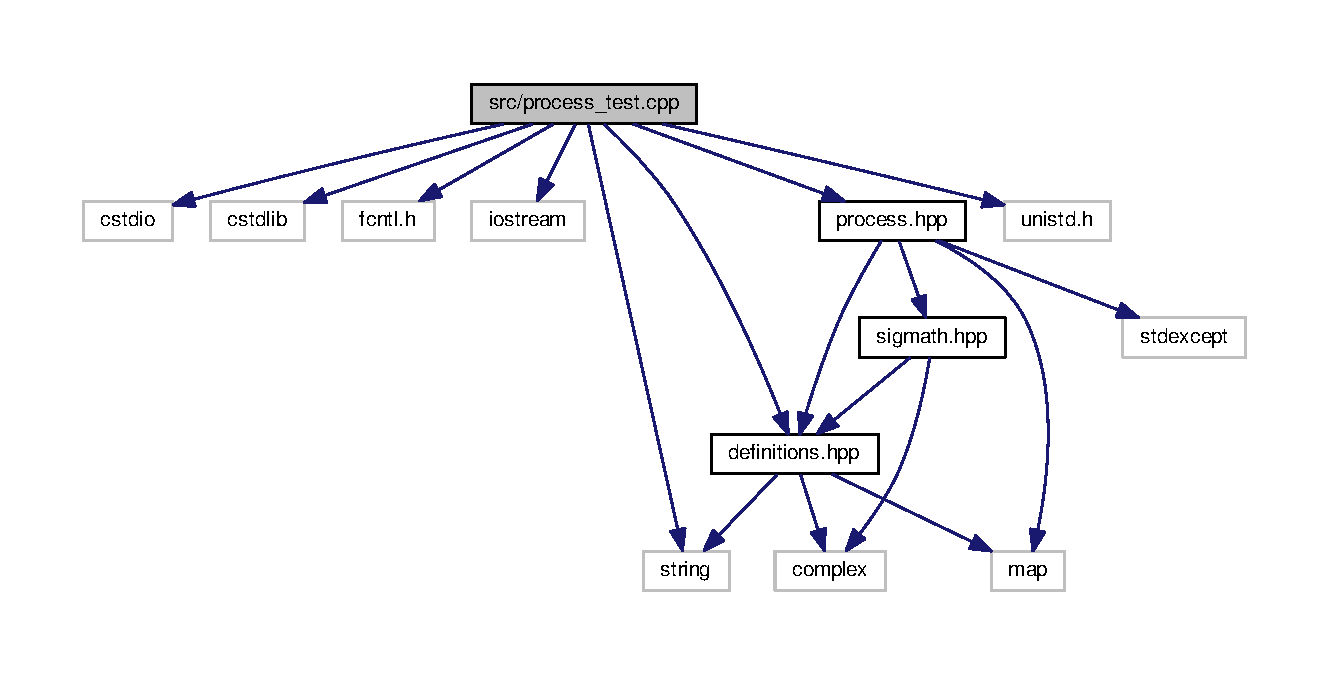
\includegraphics[width=350pt]{process__test_8cpp__incl}
\end{center}
\end{figure}
\subsection*{Macros}
\begin{DoxyCompactItemize}
\item 
\#define \hyperlink{process__test_8cpp_a698c124f1c293f98840449d6c5b9d984}{C\+O\+U\+N\+T}~131072
\end{DoxyCompactItemize}
\subsection*{Functions}
\begin{DoxyCompactItemize}
\item 
int \hyperlink{process__test_8cpp_a3c04138a5bfe5d72780bb7e82a18e627}{main} (int argc, char $\ast$$\ast$argv)
\end{DoxyCompactItemize}


\subsection{Detailed Description}
\begin{DoxyAuthor}{Author}
Samuel Andrew Wisner, \href{mailto:awisner94@gmail.com}{\tt awisner94@gmail.\+com} 

Nicholas K. Nolan 
\end{DoxyAuthor}


Definition in file \hyperlink{process__test_8cpp_source}{process\+\_\+test.\+cpp}.



\subsection{Macro Definition Documentation}
\hypertarget{process__test_8cpp_a698c124f1c293f98840449d6c5b9d984}{\index{process\+\_\+test.\+cpp@{process\+\_\+test.\+cpp}!C\+O\+U\+N\+T@{C\+O\+U\+N\+T}}
\index{C\+O\+U\+N\+T@{C\+O\+U\+N\+T}!process\+\_\+test.\+cpp@{process\+\_\+test.\+cpp}}
\subsubsection[{C\+O\+U\+N\+T}]{\setlength{\rightskip}{0pt plus 5cm}\#define C\+O\+U\+N\+T~131072}}\label{process__test_8cpp_a698c124f1c293f98840449d6c5b9d984}


Definition at line \hyperlink{process__test_8cpp_source_l00018}{18} of file \hyperlink{process__test_8cpp_source}{process\+\_\+test.\+cpp}.



\subsection{Function Documentation}
\hypertarget{process__test_8cpp_a3c04138a5bfe5d72780bb7e82a18e627}{\index{process\+\_\+test.\+cpp@{process\+\_\+test.\+cpp}!main@{main}}
\index{main@{main}!process\+\_\+test.\+cpp@{process\+\_\+test.\+cpp}}
\subsubsection[{main}]{\setlength{\rightskip}{0pt plus 5cm}int main (
\begin{DoxyParamCaption}
\item[{int}]{argc, }
\item[{char $\ast$$\ast$}]{argv}
\end{DoxyParamCaption}
)}}\label{process__test_8cpp_a3c04138a5bfe5d72780bb7e82a18e627}


Definition at line \hyperlink{process__test_8cpp_source_l00026}{26} of file \hyperlink{process__test_8cpp_source}{process\+\_\+test.\+cpp}.



Here is the call graph for this function\+:
\nopagebreak
\begin{figure}[H]
\begin{center}
\leavevmode
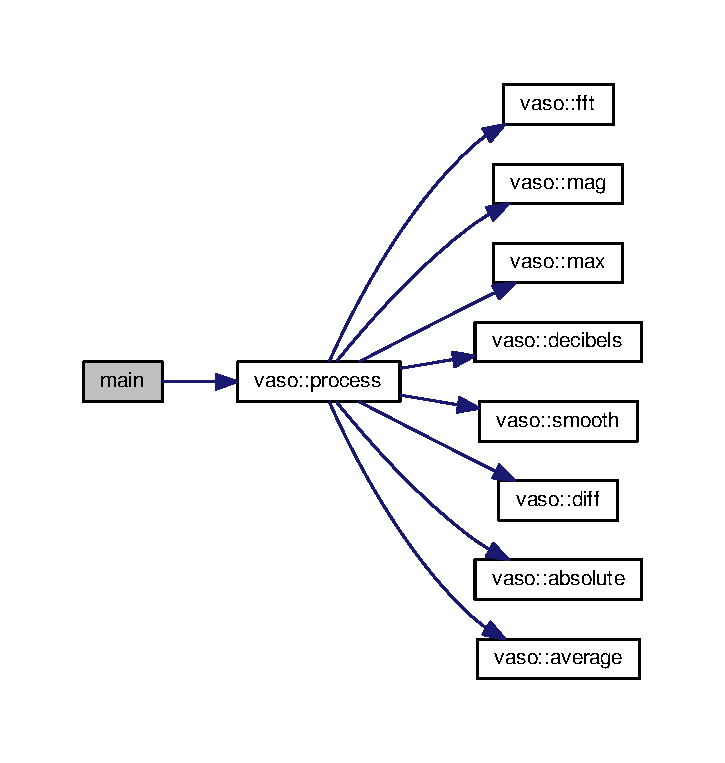
\includegraphics[width=348pt]{process__test_8cpp_a3c04138a5bfe5d72780bb7e82a18e627_cgraph}
\end{center}
\end{figure}



\hypertarget{process__test_8cpp_source}{\section{process\+\_\+test.\+cpp}
\label{process__test_8cpp_source}\index{src/process\+\_\+test.\+cpp@{src/process\+\_\+test.\+cpp}}
}

\begin{DoxyCode}
00001 
00008 \textcolor{preprocessor}{#include <cstdio>}
00009 \textcolor{preprocessor}{#include <cstdlib>}
00010 \textcolor{preprocessor}{#include <fcntl.h>}
00011 \textcolor{preprocessor}{#include <iostream>}
00012 \textcolor{preprocessor}{#include <string>}
00013 \textcolor{preprocessor}{#include <unistd.h>}
00014 
00015 \textcolor{preprocessor}{#include "\hyperlink{definitions_8hpp}{definitions.hpp}"}
00016 \textcolor{preprocessor}{#include "\hyperlink{process_8hpp}{process.hpp}"}
00017 
\hypertarget{process__test_8cpp_source_l00018}{}\hyperlink{process__test_8cpp_a698c124f1c293f98840449d6c5b9d984}{00018} \textcolor{preprocessor}{#define COUNT 131072}
00019 
00020 \textcolor{keyword}{using namespace }\hyperlink{namespacestd}{std};
00021 \textcolor{keyword}{using namespace }\hyperlink{namespacevaso}{vaso};
00022 
\hypertarget{process__test_8cpp_source_l00026}{}\hyperlink{process__test_8cpp_a3c04138a5bfe5d72780bb7e82a18e627}{00026} \textcolor{keywordtype}{int} \hyperlink{process__test_8cpp_a3c04138a5bfe5d72780bb7e82a18e627}{main}(\textcolor{keywordtype}{int} argc, \textcolor{keywordtype}{char}** argv) \{
00027     \textcolor{keywordtype}{int} file = open(\textcolor{stringliteral}{"/home/pi/vaso/etc/audio/test.raw"}, O\_RDONLY);
00028 
00029     \textcolor{keywordflow}{if}(file < 0) \{
00030         cerr << \textcolor{stringliteral}{"File unreadable!"} << endl;
00031         \textcolor{keywordflow}{return} -1;
00032     \}
00033 
00034     \hyperlink{definitions_8hpp_aacdc525d6f7bddb3ae95d5c311bd06a1}{float32}* buffer = (\hyperlink{definitions_8hpp_aacdc525d6f7bddb3ae95d5c311bd06a1}{float32}*)malloc(\hyperlink{process__test_8cpp_a698c124f1c293f98840449d6c5b9d984}{COUNT} * \textcolor{keyword}{sizeof}(\hyperlink{definitions_8hpp_aacdc525d6f7bddb3ae95d5c311bd06a1}{float32}));
00035     \textcolor{keywordtype}{int} charRead = read(file, buffer, \hyperlink{process__test_8cpp_a698c124f1c293f98840449d6c5b9d984}{COUNT} * \textcolor{keyword}{sizeof}(\hyperlink{definitions_8hpp_aacdc525d6f7bddb3ae95d5c311bd06a1}{float32}));
00036 
00037     \textcolor{keywordflow}{if}(charRead < \hyperlink{process__test_8cpp_a698c124f1c293f98840449d6c5b9d984}{COUNT}) \{
00038         cerr << \textcolor{stringliteral}{"Too few bytes read!"} << endl;
00039         \textcolor{keywordflow}{return} -1;
00040     \}
00041 
00042     close(file);
00043 
00044     \hyperlink{structDataParams}{DataParams} params = \hyperlink{namespacevaso_a8136a2891983f7a41768330e018e3232}{process}(buffer, \hyperlink{process__test_8cpp_a698c124f1c293f98840449d6c5b9d984}{COUNT}, \hyperlink{definitions_8hpp_a8ace559345ecba7978591ac2ef22aea4}{SAMPLE\_FREQ});
00045     free(buffer);
00046     cout << \textcolor{stringliteral}{"Cutoff: "} << params.\hyperlink{structDataParams_a12566e017407647bc8287d62554ad3fb}{freq} << endl;
00047     cout << \textcolor{stringliteral}{"Noise: "} << params.\hyperlink{structDataParams_a4efd1d2231c6fa7c878c9d5e1650738f}{noise} << endl;
00048 \}
\end{DoxyCode}

\hypertarget{sigmath_8hpp}{\section{src/sigmath.hpp File Reference}
\label{sigmath_8hpp}\index{src/sigmath.\+hpp@{src/sigmath.\+hpp}}
}
{\ttfamily \#include $<$complex$>$}\\*
{\ttfamily \#include \char`\"{}definitions.\+hpp\char`\"{}}\\*
Include dependency graph for sigmath.\+hpp\+:
\nopagebreak
\begin{figure}[H]
\begin{center}
\leavevmode
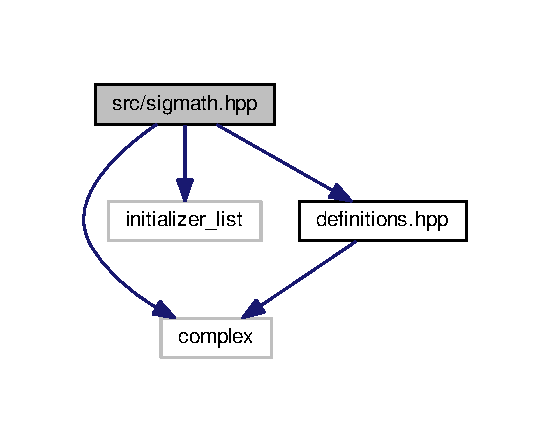
\includegraphics[width=197pt]{sigmath_8hpp__incl}
\end{center}
\end{figure}
This graph shows which files directly or indirectly include this file\+:
\nopagebreak
\begin{figure}[H]
\begin{center}
\leavevmode
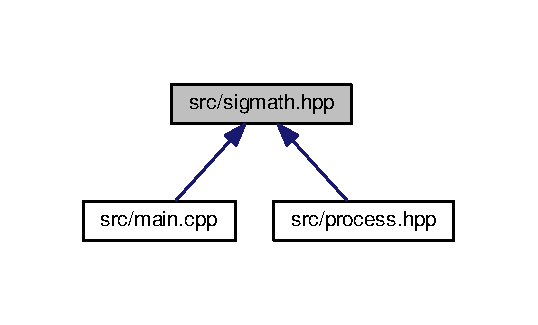
\includegraphics[width=258pt]{sigmath_8hpp__dep__incl}
\end{center}
\end{figure}
\subsection*{Namespaces}
\begin{DoxyCompactItemize}
\item 
 \hyperlink{namespacevaso}{vaso}
\begin{DoxyCompactList}\small\item\em contains functions related to the file I/\+O use in this program \end{DoxyCompactList}\end{DoxyCompactItemize}
\subsection*{Functions}
\begin{DoxyCompactItemize}
\item 
void \hyperlink{namespacevaso_a6ca90add966ce1773fc59a6883e6cd0c}{vaso\+::absolute} (\hyperlink{definitions_8hpp_aacdc525d6f7bddb3ae95d5c311bd06a1}{float32} $\ast$data, \hyperlink{definitions_8hpp_a1134b580f8da4de94ca6b1de4d37975e}{uint32} size)
\item 
\hyperlink{definitions_8hpp_aacdc525d6f7bddb3ae95d5c311bd06a1}{float32} \hyperlink{namespacevaso_ad3205136b1cd04b4c6b9d7be73661796}{vaso\+::average} (\hyperlink{definitions_8hpp_aacdc525d6f7bddb3ae95d5c311bd06a1}{float32} $\ast$data, \hyperlink{definitions_8hpp_a1134b580f8da4de94ca6b1de4d37975e}{uint32} size)
\item 
\hyperlink{structDataParams}{Data\+Params} \hyperlink{namespacevaso_a376413e791defec04a0faf329be1cbf4}{vaso\+::average} (\hyperlink{structDataParams}{Data\+Params} $\ast$params, \hyperlink{definitions_8hpp_adde6aaee8457bee49c2a92621fe22b79}{uint8} size)
\item 
void \hyperlink{namespacevaso_a9d0e5d69685ee494d286db6ece005156}{vaso\+::average} (\hyperlink{definitions_8hpp_aacdc525d6f7bddb3ae95d5c311bd06a1}{float32} $\ast$data, \hyperlink{definitions_8hpp_aacdc525d6f7bddb3ae95d5c311bd06a1}{float32} $\ast$avg, \hyperlink{definitions_8hpp_adde6aaee8457bee49c2a92621fe22b79}{uint8} count, \hyperlink{definitions_8hpp_a1134b580f8da4de94ca6b1de4d37975e}{uint32} size)
\item 
void \hyperlink{namespacevaso_af9bb2211cf3478333dfc1873bf316263}{vaso\+::decibels} (\hyperlink{definitions_8hpp_aacdc525d6f7bddb3ae95d5c311bd06a1}{float32} $\ast$data, \hyperlink{definitions_8hpp_a1134b580f8da4de94ca6b1de4d37975e}{uint32} size)
\item 
void \hyperlink{namespacevaso_a7d108bce812e906d8b1810815774c7ea}{vaso\+::diff} (\hyperlink{definitions_8hpp_aacdc525d6f7bddb3ae95d5c311bd06a1}{float32} $\ast$data, \hyperlink{definitions_8hpp_a1134b580f8da4de94ca6b1de4d37975e}{uint32} size)
\item 
void \hyperlink{namespacevaso_af74f08a8afd7967b6c2b3c2b0e5fb1e9}{vaso\+::fft} (\hyperlink{definitions_8hpp_a960be6b6614c08090c16574dba10a421}{cfloat32} $\ast$data, \hyperlink{definitions_8hpp_a1134b580f8da4de94ca6b1de4d37975e}{uint32} size)
\item 
void \hyperlink{namespacevaso_a5d355b5c326a852e2ce95c258450898c}{vaso\+::mag} (\hyperlink{definitions_8hpp_a960be6b6614c08090c16574dba10a421}{cfloat32} $\ast$orig, \hyperlink{definitions_8hpp_aacdc525d6f7bddb3ae95d5c311bd06a1}{float32} $\ast$newmags, \hyperlink{definitions_8hpp_a1134b580f8da4de94ca6b1de4d37975e}{uint32} size)
\item 
\hyperlink{structMaximum}{Maximum} \hyperlink{namespacevaso_a122846d728be312454a452d379915e10}{vaso\+::max} (\hyperlink{definitions_8hpp_aacdc525d6f7bddb3ae95d5c311bd06a1}{float32} $\ast$data, \hyperlink{definitions_8hpp_a1134b580f8da4de94ca6b1de4d37975e}{uint32} size)
\item 
void \hyperlink{namespacevaso_a5b7fc1a58199e2cac989f417a9faa1ce}{vaso\+::smooth} (\hyperlink{definitions_8hpp_aacdc525d6f7bddb3ae95d5c311bd06a1}{float32} $\ast$data, \hyperlink{definitions_8hpp_a1134b580f8da4de94ca6b1de4d37975e}{uint32} size, \hyperlink{definitions_8hpp_a05f6b0ae8f6a6e135b0e290c25fe0e4e}{uint16} order)
\end{DoxyCompactItemize}

\hypertarget{sigmath_8hpp_source}{\section{sigmath.\+hpp}
\label{sigmath_8hpp_source}\index{src/sigmath.\+hpp@{src/sigmath.\+hpp}}
}

\begin{DoxyCode}
00001 
00008 \textcolor{preprocessor}{#ifndef sigmath\_H}
00009 \textcolor{preprocessor}{#define sigmath\_H}
00010 
00011 \textcolor{preprocessor}{#include <complex>}
00012 
00013 \textcolor{preprocessor}{#include "\hyperlink{definitions_8hpp}{definitions.hpp}"}
00014 
00015 \textcolor{keyword}{namespace }\hyperlink{namespacevaso}{vaso} \{
00016     \textcolor{comment}{// PROTOTYPES}
00017 
00026     \textcolor{keywordtype}{void} \hyperlink{namespacevaso_a6ca90add966ce1773fc59a6883e6cd0c}{absolute}(\hyperlink{definitions_8hpp_aacdc525d6f7bddb3ae95d5c311bd06a1}{float32}* data, \hyperlink{definitions_8hpp_a1134b580f8da4de94ca6b1de4d37975e}{uint32} size);
00027 
00037     \hyperlink{definitions_8hpp_aacdc525d6f7bddb3ae95d5c311bd06a1}{float32} \hyperlink{namespacevaso_ad3205136b1cd04b4c6b9d7be73661796}{average}(\hyperlink{definitions_8hpp_aacdc525d6f7bddb3ae95d5c311bd06a1}{float32}* data, \hyperlink{definitions_8hpp_a1134b580f8da4de94ca6b1de4d37975e}{uint32} size);
00038 
00049     \hyperlink{structDataParams}{DataParams} \hyperlink{namespacevaso_ad3205136b1cd04b4c6b9d7be73661796}{average}(\hyperlink{structDataParams}{DataParams}* params, \hyperlink{definitions_8hpp_adde6aaee8457bee49c2a92621fe22b79}{uint8} size);
00050 
00067     \textcolor{keywordtype}{void} \hyperlink{namespacevaso_ad3205136b1cd04b4c6b9d7be73661796}{average}(\hyperlink{definitions_8hpp_aacdc525d6f7bddb3ae95d5c311bd06a1}{float32}* data, \hyperlink{definitions_8hpp_aacdc525d6f7bddb3ae95d5c311bd06a1}{float32}* avg, \hyperlink{definitions_8hpp_adde6aaee8457bee49c2a92621fe22b79}{uint8} count, 
      \hyperlink{definitions_8hpp_a1134b580f8da4de94ca6b1de4d37975e}{uint32} size);
00068 
00080     \textcolor{keywordtype}{void} \hyperlink{namespacevaso_af9bb2211cf3478333dfc1873bf316263}{decibels}(\hyperlink{definitions_8hpp_aacdc525d6f7bddb3ae95d5c311bd06a1}{float32}* data, \hyperlink{definitions_8hpp_a1134b580f8da4de94ca6b1de4d37975e}{uint32} size);
00081 
00090     \textcolor{keywordtype}{void} \hyperlink{namespacevaso_a7d108bce812e906d8b1810815774c7ea}{diff}(\hyperlink{definitions_8hpp_aacdc525d6f7bddb3ae95d5c311bd06a1}{float32}* data, \hyperlink{definitions_8hpp_a1134b580f8da4de94ca6b1de4d37975e}{uint32} size);
00091 
00103     \textcolor{keywordtype}{void} \hyperlink{namespacevaso_af74f08a8afd7967b6c2b3c2b0e5fb1e9}{fft}(\hyperlink{definitions_8hpp_a960be6b6614c08090c16574dba10a421}{cfloat32}* data, \hyperlink{definitions_8hpp_a1134b580f8da4de94ca6b1de4d37975e}{uint32} size);
00104 
00114     \textcolor{keywordtype}{void} \hyperlink{namespacevaso_a5d355b5c326a852e2ce95c258450898c}{mag}(\hyperlink{definitions_8hpp_a960be6b6614c08090c16574dba10a421}{cfloat32}* orig, \hyperlink{definitions_8hpp_aacdc525d6f7bddb3ae95d5c311bd06a1}{float32}* newmags, \hyperlink{definitions_8hpp_a1134b580f8da4de94ca6b1de4d37975e}{uint32} size);
00115 
00125     \hyperlink{structMaximum}{Maximum} \hyperlink{namespacevaso_a122846d728be312454a452d379915e10}{max}(\hyperlink{definitions_8hpp_aacdc525d6f7bddb3ae95d5c311bd06a1}{float32}* data, \hyperlink{definitions_8hpp_a1134b580f8da4de94ca6b1de4d37975e}{uint32} size);
00126 
00137     \textcolor{keywordtype}{void} \hyperlink{namespacevaso_a5b7fc1a58199e2cac989f417a9faa1ce}{smooth}(\hyperlink{definitions_8hpp_aacdc525d6f7bddb3ae95d5c311bd06a1}{float32}* data, \hyperlink{definitions_8hpp_a1134b580f8da4de94ca6b1de4d37975e}{uint32} size, \hyperlink{definitions_8hpp_a05f6b0ae8f6a6e135b0e290c25fe0e4e}{uint16} order);
00138 
00139     \textcolor{comment}{// DEFINITIONS}
00140 
\hypertarget{sigmath_8hpp_source_l00141}{}\hyperlink{namespacevaso_a6ca90add966ce1773fc59a6883e6cd0c}{00141}     \textcolor{keywordtype}{void} \hyperlink{namespacevaso_a6ca90add966ce1773fc59a6883e6cd0c}{absolute}(\hyperlink{definitions_8hpp_aacdc525d6f7bddb3ae95d5c311bd06a1}{float32}* data, \hyperlink{definitions_8hpp_a1134b580f8da4de94ca6b1de4d37975e}{uint32} size) \{
00142 
00143     \}
00144 
\hypertarget{sigmath_8hpp_source_l00145}{}\hyperlink{namespacevaso_ad3205136b1cd04b4c6b9d7be73661796}{00145}     \hyperlink{definitions_8hpp_aacdc525d6f7bddb3ae95d5c311bd06a1}{float32} \hyperlink{namespacevaso_ad3205136b1cd04b4c6b9d7be73661796}{average}(\hyperlink{definitions_8hpp_aacdc525d6f7bddb3ae95d5c311bd06a1}{float32}* data, \hyperlink{definitions_8hpp_a1134b580f8da4de94ca6b1de4d37975e}{uint32} size) \{
00146 
00147     \}
00148 
\hypertarget{sigmath_8hpp_source_l00149}{}\hyperlink{namespacevaso_a376413e791defec04a0faf329be1cbf4}{00149}     \hyperlink{structDataParams}{DataParams} \hyperlink{namespacevaso_ad3205136b1cd04b4c6b9d7be73661796}{average}(\hyperlink{structDataParams}{DataParams}* params, \hyperlink{definitions_8hpp_adde6aaee8457bee49c2a92621fe22b79}{uint8} size) \{
00150 
00151     \}
00152 
\hypertarget{sigmath_8hpp_source_l00153}{}\hyperlink{namespacevaso_a9d0e5d69685ee494d286db6ece005156}{00153}     \textcolor{keywordtype}{void} \hyperlink{namespacevaso_ad3205136b1cd04b4c6b9d7be73661796}{average}(\hyperlink{definitions_8hpp_aacdc525d6f7bddb3ae95d5c311bd06a1}{float32}* data, \hyperlink{definitions_8hpp_aacdc525d6f7bddb3ae95d5c311bd06a1}{float32}* avg, \hyperlink{definitions_8hpp_adde6aaee8457bee49c2a92621fe22b79}{uint8} count, 
      \hyperlink{definitions_8hpp_a1134b580f8da4de94ca6b1de4d37975e}{uint32} size) \{
00154         \textcolor{comment}{// data is an array. Access like so: data[index]}
00155     \}
00156 
\hypertarget{sigmath_8hpp_source_l00157}{}\hyperlink{namespacevaso_af9bb2211cf3478333dfc1873bf316263}{00157}     \textcolor{keywordtype}{void} \hyperlink{namespacevaso_af9bb2211cf3478333dfc1873bf316263}{decibels}(\hyperlink{definitions_8hpp_aacdc525d6f7bddb3ae95d5c311bd06a1}{float32}* data, \hyperlink{definitions_8hpp_a1134b580f8da4de94ca6b1de4d37975e}{uint32} size) \{
00158         \textcolor{keywordflow}{for}(\hyperlink{definitions_8hpp_a1134b580f8da4de94ca6b1de4d37975e}{uint32} i = 0; i < size; i++) \{
00159             data[i] = 20 * log10(data[i]);
00160         \}
00161     \}
00162 
\hypertarget{sigmath_8hpp_source_l00163}{}\hyperlink{namespacevaso_a7d108bce812e906d8b1810815774c7ea}{00163}     \textcolor{keywordtype}{void} \hyperlink{namespacevaso_a7d108bce812e906d8b1810815774c7ea}{diff}(\hyperlink{definitions_8hpp_aacdc525d6f7bddb3ae95d5c311bd06a1}{float32}* data, \hyperlink{definitions_8hpp_a1134b580f8da4de94ca6b1de4d37975e}{uint32} size) \{
00164 
00165     \}
00166 
\hypertarget{sigmath_8hpp_source_l00167}{}\hyperlink{namespacevaso_af74f08a8afd7967b6c2b3c2b0e5fb1e9}{00167}     \textcolor{keywordtype}{void} \hyperlink{namespacevaso_af74f08a8afd7967b6c2b3c2b0e5fb1e9}{fft}(\hyperlink{definitions_8hpp_a960be6b6614c08090c16574dba10a421}{cfloat32}* data, \hyperlink{definitions_8hpp_a1134b580f8da4de94ca6b1de4d37975e}{uint32} size) \{
00168         \textcolor{comment}{// DFT}
00169         \hyperlink{definitions_8hpp_a1134b580f8da4de94ca6b1de4d37975e}{uint32} k = size;
00170         \hyperlink{definitions_8hpp_a1134b580f8da4de94ca6b1de4d37975e}{uint32} n;
00171         \hyperlink{definitions_8hpp_aacdc525d6f7bddb3ae95d5c311bd06a1}{float32} thetaT = M\_PI / size;
00172         \hyperlink{definitions_8hpp_a960be6b6614c08090c16574dba10a421}{cfloat32} phiT(cos(thetaT), sin(thetaT));
00173         \hyperlink{definitions_8hpp_a960be6b6614c08090c16574dba10a421}{cfloat32} T;
00174 
00175         \textcolor{keywordflow}{while}(k > 1) \{
00176             n = k;
00177             k >>= 1;
00178             phiT = phiT * phiT;
00179             T = 1.0L;
00180 
00181             \textcolor{keywordflow}{for}(\hyperlink{definitions_8hpp_a1134b580f8da4de94ca6b1de4d37975e}{uint32} l = 0; l < k; l++) \{
00182                 \textcolor{keywordflow}{for}(\hyperlink{definitions_8hpp_a1134b580f8da4de94ca6b1de4d37975e}{uint32} a = l; a < size; a += n) \{
00183                     \hyperlink{definitions_8hpp_a1134b580f8da4de94ca6b1de4d37975e}{uint32} b = a + k;
00184                     \hyperlink{definitions_8hpp_a960be6b6614c08090c16574dba10a421}{cfloat32} t = data[a] -data[b];
00185                     data[a] +=data[b];
00186                     data[b] = t * T;
00187                 \}
00188 
00189                 T *= phiT;
00190             \}
00191         \}
00192 
00193         \textcolor{comment}{// Decimate}
00194         \hyperlink{definitions_8hpp_a1134b580f8da4de94ca6b1de4d37975e}{uint32} m = (\hyperlink{definitions_8hpp_a1134b580f8da4de94ca6b1de4d37975e}{uint32})log2(size);
00195 
00196         \textcolor{keywordflow}{for}(\hyperlink{definitions_8hpp_a1134b580f8da4de94ca6b1de4d37975e}{uint32} a = 0; a < size; a++) \{
00197             \hyperlink{definitions_8hpp_a1134b580f8da4de94ca6b1de4d37975e}{uint32} b = a;
00198 
00199             \textcolor{comment}{// Reverse bits}
00200             b = (((b & 0xaaaaaaaa) >> 1) | ((b & 0x55555555) << 1));
00201             b = (((b & 0xcccccccc) >> 2) | ((b & 0x33333333) << 2));
00202             b = (((b & 0xf0f0f0f0) >> 4) | ((b & 0x0f0f0f0f) << 4));
00203             b = (((b & 0xff00ff00) >> 8) | ((b & 0x00ff00ff) << 8));
00204             b = ((b >> 16) | (b << 16)) >> (32 - m);
00205 
00206             \textcolor{keywordflow}{if} (b > a)
00207             \{
00208                 \hyperlink{definitions_8hpp_a960be6b6614c08090c16574dba10a421}{cfloat32} t = data[a];
00209                 data[a] =data[b];
00210                 data[b] = t;
00211             \}
00212         \}
00213     \}
00214 
\hypertarget{sigmath_8hpp_source_l00215}{}\hyperlink{namespacevaso_a5d355b5c326a852e2ce95c258450898c}{00215}     \textcolor{keywordtype}{void} \hyperlink{namespacevaso_a5d355b5c326a852e2ce95c258450898c}{mag}(\hyperlink{definitions_8hpp_a960be6b6614c08090c16574dba10a421}{cfloat32}* orig, \hyperlink{definitions_8hpp_aacdc525d6f7bddb3ae95d5c311bd06a1}{float32}* newmags, \hyperlink{definitions_8hpp_a1134b580f8da4de94ca6b1de4d37975e}{uint32} size) \{
00216 
00217     \}
00218 
\hypertarget{sigmath_8hpp_source_l00219}{}\hyperlink{namespacevaso_a122846d728be312454a452d379915e10}{00219}     \hyperlink{structMaximum}{Maximum} \hyperlink{namespacevaso_a122846d728be312454a452d379915e10}{max}(\hyperlink{definitions_8hpp_aacdc525d6f7bddb3ae95d5c311bd06a1}{float32}* data, \hyperlink{definitions_8hpp_a1134b580f8da4de94ca6b1de4d37975e}{uint32} size) \{
00220 
00221     \}
00222 
\hypertarget{sigmath_8hpp_source_l00223}{}\hyperlink{namespacevaso_a5b7fc1a58199e2cac989f417a9faa1ce}{00223}     \textcolor{keywordtype}{void} \hyperlink{namespacevaso_a5b7fc1a58199e2cac989f417a9faa1ce}{smooth}(\hyperlink{definitions_8hpp_aacdc525d6f7bddb3ae95d5c311bd06a1}{float32}* data, \hyperlink{definitions_8hpp_a1134b580f8da4de94ca6b1de4d37975e}{uint32} size, \hyperlink{definitions_8hpp_a05f6b0ae8f6a6e135b0e290c25fe0e4e}{uint16} order) \{
00224         \hyperlink{definitions_8hpp_aacdc525d6f7bddb3ae95d5c311bd06a1}{float32} coeff = 1 / (\hyperlink{definitions_8hpp_aacdc525d6f7bddb3ae95d5c311bd06a1}{float32})order;
00225         \hyperlink{definitions_8hpp_aacdc525d6f7bddb3ae95d5c311bd06a1}{float32} temp[size];
00226 
00227         \textcolor{keywordflow}{for}(\hyperlink{definitions_8hpp_a1134b580f8da4de94ca6b1de4d37975e}{uint32} i = 0; i < size; i++) \{
00228             temp[i] = 0;
00229 
00230             \textcolor{keywordflow}{for}(\hyperlink{definitions_8hpp_a05f6b0ae8f6a6e135b0e290c25fe0e4e}{uint16} j = 0; j < order && j <= i; j++) \{
00231                 temp[i] += data[i - j];
00232             \}
00233 
00234             temp[i] *= coeff;
00235         \}
00236     \}
00237 \}
00238 
00239 \textcolor{preprocessor}{#endif}
\end{DoxyCode}

\hypertarget{sigmath__test_8cpp}{\section{src/sigmath\+\_\+test.cpp File Reference}
\label{sigmath__test_8cpp}\index{src/sigmath\+\_\+test.\+cpp@{src/sigmath\+\_\+test.\+cpp}}
}
{\ttfamily \#include $<$string$>$}\\*
{\ttfamily \#include \char`\"{}definitions.\+hpp\char`\"{}}\\*
{\ttfamily \#include \char`\"{}fileio.\+hpp\char`\"{}}\\*
{\ttfamily \#include \char`\"{}process.\+hpp\char`\"{}}\\*
Include dependency graph for sigmath\+\_\+test.\+cpp\+:
\nopagebreak
\begin{figure}[H]
\begin{center}
\leavevmode
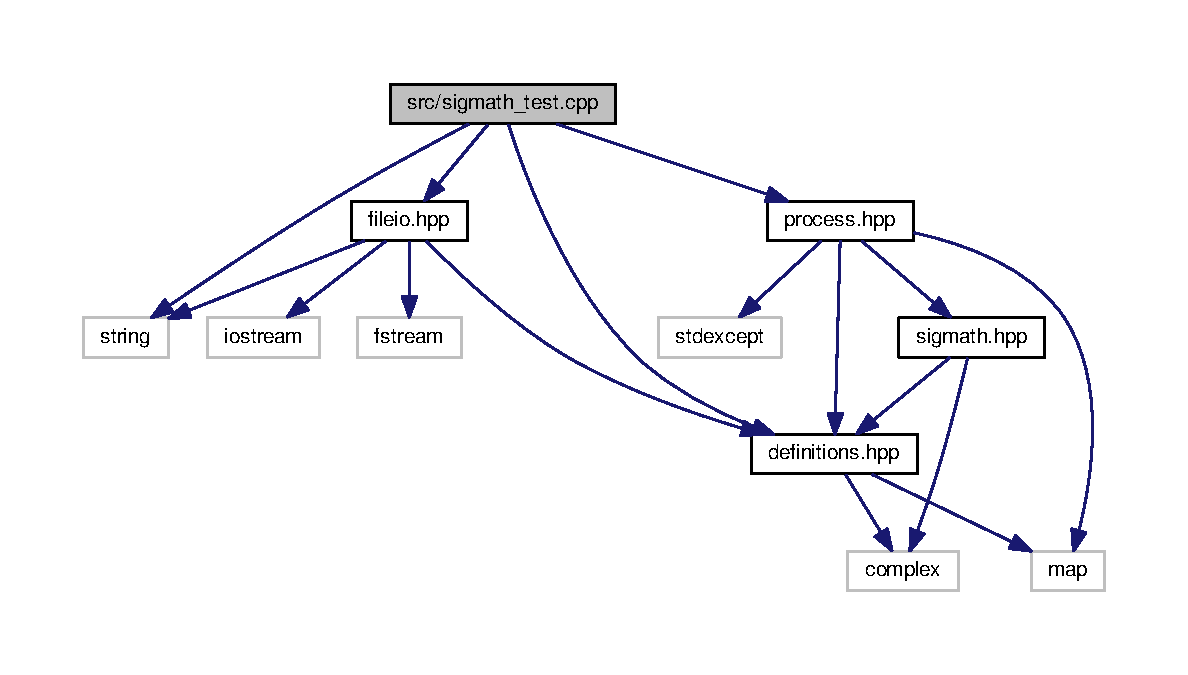
\includegraphics[width=350pt]{sigmath__test_8cpp__incl}
\end{center}
\end{figure}
\subsection*{Functions}
\begin{DoxyCompactItemize}
\item 
int \hyperlink{sigmath__test_8cpp_a3c04138a5bfe5d72780bb7e82a18e627}{main} (int argc, char $\ast$$\ast$argv)
\end{DoxyCompactItemize}


\subsection{Function Documentation}
\hypertarget{sigmath__test_8cpp_a3c04138a5bfe5d72780bb7e82a18e627}{\index{sigmath\+\_\+test.\+cpp@{sigmath\+\_\+test.\+cpp}!main@{main}}
\index{main@{main}!sigmath\+\_\+test.\+cpp@{sigmath\+\_\+test.\+cpp}}
\subsubsection[{main}]{\setlength{\rightskip}{0pt plus 5cm}int main (
\begin{DoxyParamCaption}
\item[{int}]{argc, }
\item[{char $\ast$$\ast$}]{argv}
\end{DoxyParamCaption}
)}}\label{sigmath__test_8cpp_a3c04138a5bfe5d72780bb7e82a18e627}


Definition at line \hyperlink{sigmath__test_8cpp_source_l00020}{20} of file \hyperlink{sigmath__test_8cpp_source}{sigmath\+\_\+test.\+cpp}.


\hypertarget{sigmath__test_8cpp_source}{\section{sigmath\+\_\+test.\+cpp}
\label{sigmath__test_8cpp_source}\index{src/sigmath\+\_\+test.\+cpp@{src/sigmath\+\_\+test.\+cpp}}
}

\begin{DoxyCode}
00001 
00007 \textcolor{preprocessor}{#include <string>}
00008 
00009 \textcolor{preprocessor}{#include "\hyperlink{definitions_8hpp}{definitions.hpp}"}
00010 \textcolor{preprocessor}{#include "\hyperlink{fileio_8hpp}{fileio.hpp}"}
00011 \textcolor{preprocessor}{#include "\hyperlink{process_8hpp}{process.hpp}"}
00012 
00013 \textcolor{keyword}{using namespace }\hyperlink{namespacestd}{std};
00014 \textcolor{keyword}{using namespace }\hyperlink{namespacevaso}{vaso};
00015 
\hypertarget{sigmath__test_8cpp_source_l00020}{}\hyperlink{sigmath__test_8cpp_a3c04138a5bfe5d72780bb7e82a18e627}{00020} \textcolor{keywordtype}{int} \hyperlink{sigmath__test_8cpp_a3c04138a5bfe5d72780bb7e82a18e627}{main}(\textcolor{keywordtype}{int} argc, \textcolor{keywordtype}{char}** argv) \{
00021 
00022 \}
\end{DoxyCode}

\hypertarget{sound_8hpp}{\section{src/sound.hpp File Reference}
\label{sound_8hpp}\index{src/sound.\+hpp@{src/sound.\+hpp}}
}
{\ttfamily \#include $<$string$>$}\\*
{\ttfamily \#include \char`\"{}definitions.\+hpp\char`\"{}}\\*
Include dependency graph for sound.\+hpp\+:
\nopagebreak
\begin{figure}[H]
\begin{center}
\leavevmode
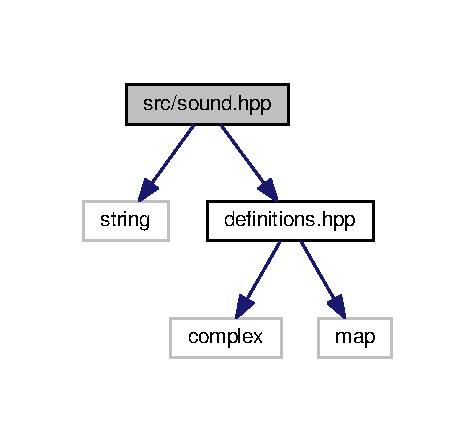
\includegraphics[width=220pt]{sound_8hpp__incl}
\end{center}
\end{figure}
\subsection*{Namespaces}
\begin{DoxyCompactItemize}
\item 
 \hyperlink{namespacevaso}{vaso}
\begin{DoxyCompactList}\small\item\em contains functions related to the file I/\+O use in this program \end{DoxyCompactList}\end{DoxyCompactItemize}
\subsection*{Functions}
\begin{DoxyCompactItemize}
\item 
void \hyperlink{namespacevaso_a7da499b9b1b5a492bea8ab8681e57c22}{vaso\+::play} (auto filename)
\end{DoxyCompactItemize}

\hypertarget{sound_8hpp_source}{\section{sound.\+hpp}
\label{sound_8hpp_source}\index{src/sound.\+hpp@{src/sound.\+hpp}}
}

\begin{DoxyCode}
00001 
00007 \textcolor{preprocessor}{#ifndef sound\_H}
00008 \textcolor{preprocessor}{#define sound\_H}
00009 
00010 \textcolor{preprocessor}{#include <string>}
00011 
00012 \textcolor{preprocessor}{#include "\hyperlink{definitions_8hpp}{definitions.hpp}"}
00013 
00014 \textcolor{keyword}{namespace }\hyperlink{namespaceavda}{avda} \{
\hypertarget{sound_8hpp_source_l00020}{}\hyperlink{namespaceavda_a34f661f9a357bb68b0aa3662cc821e4d}{00020}     \textcolor{keywordtype}{void} \hyperlink{namespaceavda_a34f661f9a357bb68b0aa3662cc821e4d}{play}(\textcolor{keyword}{auto} filename) \{
00021 
00022     \}
00023 \}
00024 
00025 \textcolor{preprocessor}{#endif}
\end{DoxyCode}

%--- End generated contents ---

% Index
\newpage
\phantomsection
\addcontentsline{toc}{chapter}{Index}
\printindex

\end{document}
